%%%%%%%%%%%%%%%%%%%%%%%%%%%%%%%%%%%%%%%%%%%PHYSICS 137A NOTES%%%%%%%%%%%%%%%%%%%%%%%%%%%%%%%%%%%%%%%%%%%%%%%%%%
%%PACKAGE INCLUSIONS%%
\documentclass{book}
\usepackage[letterpaper, margin=1in]{geometry}
\usepackage[pdftex]{graphicx}
\usepackage[utf8]{inputenc}
\usepackage{tikz, pgfplots, wrapfig, amssymb, array, mathtools, enumitem, circuitikz, physics, parskip, hyperref}
\usepackage{tkz-euclide}
\usepackage{titlesec}
\usepackage{lipsum}
\usepackage[english]{babel}
\usepackage{amsmath, amsthm}
\usepackage{fancyhdr}
\usepackage{xcoffins}
\usepackage{dirtytalk}
\usepackage{shortcuts}

\theoremstyle{plain}
\usetikzlibrary{calc,patterns,angles,quotes}
\setlength{\parskip}{0pt}
\usetikzlibrary{calc,patterns,angles,quotes}
\makeatletter
\pagestyle{fancy}
\setlength{\parskip}{1ex plus 0.5ex minus 0.2ex}
\pgfplotsset{compat=1.17}
%%%%%%%%%%%%%%%%%%%%%%%%%%%%%%%%%%%%%%%%%%%%%%%%%%%%%%%%%%%%%%%%%%%%%%%%%%%%%%%%%%%%%%%%%%%%%%%%%%%%%%%%%%%%%%%
%%SECTIONING EDITS%%
%
%DEFINITION FOR CHAPTER HEADERS%
\def\thickhrulefill{\leavevmode \leaders \hrule height 1ex \hfill \kern \z@}
\def\@makechapterhead#1{
  {\parindent \z@ \centering \reset@font
        \thickhrulefill\quad
        \scshape Lecture \thechapter
        \quad \thickhrulefill
        \par\nobreak
        \vspace*{10\p@}%
        \interlinepenalty\@M
        \hrule
        \vspace*{10\p@}%
        \huge \bfseries #1\par\nobreak
        \par
        \vspace*{10\p@}%
        \hrule
    \vskip 20\p@
  }}
%%%%%%%%%%%%%%%%%%%%%%%%%%%%%%%%%%%%%%%%%%%%%%%%%%%%%%%%%%%%%%%%%%%%%%%%%%%%%%%%%%%%%%%%%%%%%%%%%%%%
%PART STYLING%
\titleclass{\part}{top} % make part like a chapter
\titleformat{\part}
[display]
{\centering\normalfont\huge\bfseries}
{\vspace{200pt}\titlerule[5pt]\vspace{3pt}\titlerule[2pt]\vspace{3pt}\MakeUppercase{Part} \thepart}
{0pt}
{\titlerule[2pt]\vspace{20pt}\huge\MakeUppercase}

\titlespacing*{\part}{0pt}{0pt}{20pt}
%%%%%%%%%%%%%%%%%%%%%%%%%%%%%%%%%%%%%%%%%%%%%%%%%%%%%%%%%%%%%%%%%%%%%%%%%%%%%%%%%%%%%%%%%%%%%%%%%%%%
%SECTION STYLING%
\def\section{\@ifstar\unnumberedsection\numberedsection}
\def\numberedsection{\@ifnextchar[%]
    \numberedsectionwithtwoarguments\numberedsectionwithoneargument}
\def\numberedsectionwithoneargument#1{\numberedsectionwithtwoarguments[#1]{#1}}
\def\numberedsectionwithtwoarguments[#1]#2{%
    \ifhmode\par\fi
    \removelastskip
    \vskip 5ex\goodbreak
    \refstepcounter{section}%
    \hbox to \hsize{\hss\vbox{\advance\hsize by 0cm
        \noindent
        \leavevmode\Large\bfseries\raggedright
        \thesection\space$\bigg\vert$\hskip -1ex $\bigg\vert$\space   \
        #2\par
        \vskip -2ex
        \noindent\hrulefill
        \vskip -3ex
        \noindent\hrulefill
        }}\nobreak
    \vskip 2ex\nobreak
    \addcontentsline{toc}{section}{%
    \protect\numberline{\thesection}%
    #1}%
}
%%%%%%%%%%%%%%%%%%%%%%%%%%%%%%%%%%%%%%%%%%%%%%%%%%%%%%%%%%%%%%%%%%%%%%%%%%%%%%%%%%%%%%%%%%%%%%%%%%%%
%SUBSECTION STYLING%
\def\subsection{\@ifstar\unnumberedsubection\numberedsubsection}
\def\numberedsubsection{\@ifnextchar[%]
    \numberedsubsectionwithtwoarguments\numberedsubsectionwithoneargument}
\def\numberedsubsectionwithoneargument#1{\numberedsubsectionwithtwoarguments[#1]{#1}}
\def\numberedsubsectionwithtwoarguments[#1]#2{%
    \ifhmode\par\fi
    \removelastskip
    \vskip 5ex\goodbreak
    \refstepcounter{subsection}%
    \hbox to \hsize{\hss\vbox{\advance\hsize by 0cm
        \noindent
        \leavevmode\large\bfseries\raggedright
        \thesubsection\space$\bigg\vert$\space\
        #2\par
        \vskip -2ex
        \noindent\hrulefill
        }}\nobreak
    \vskip 2ex\nobreak
    \addcontentsline{toc}{subsection}{%
        \protect\numberline{\thesubsection}%
        #1}%
    }

    \makeatother
%%%%%%%%%%%%%%%%%%%%%%%%%%%%%%%%%%%%%%%%%%%%%%%%%%%%%%%%%%%%%%%%%%%%%%%%%%%%%%%%%%%%%%%%%%%%%%%%%%%%%%%%%%%%%%%
\begin{document}

  %TITLE PAGE%
  \begin{titlepage}
      \centering
      \vspace*{\baselineskip}\vspace{200pt}
      \rule{\textwidth}{1.6pt}\vspace*{-\baselineskip}\vspace*{2pt}
      \rule{\textwidth}{0.4pt}\\[\baselineskip]
      {\Huge \bfseries PHYSICS 137A NOTES}\\[0.2\baselineskip]
      \rule{\textwidth}{0.4pt}\vspace*{-\baselineskip}\vspace{3.2pt}
      \rule{\textwidth}{1.6pt}\\[\baselineskip]
      \scshape
      Typeset notes for Physics 137A: Quantum Mechanics I\\
      \par
      \vspace*{2pt}
      {\Large Andrew Binder and Eric Du}\\
      {\large University of California, Berkeley\par}
      {\scshape Fall 2022} \\
  \end{titlepage}

  \tableofcontents
  \newpage
  \setcounter{chapter}{-1}
%%%%%%%%%%%%%%%%%%%%%%%%%%%%%%%%%%%%%%%%%%%%%%%%%%%%%%%%%%%%%%%%%%%%%%%%%%%%%%%%%%%%%%%%%%%%%%%%%%%%%%%%%%%%%%%
%%%%%%%%%%%%%%%%%%%%%%%%%%%%%%%%%%%%%%%%%%%%%INTRODUCTION%%%%%%%%%%%%%%%%%%%%%%%%%%%%%%%%%%%%%%%%%%%%%%%%%%%%%%
    \chapter{Introduction}
      This course is titled \textbf{Quantum Mechanics I}. Eric and Andrew both took this course in Fall 2022.
      \section{Basic Syllabus Info}
          Here, there is some basic information regarding the syllabus for this course as it was taught in Fall 2022.
          \subsubsection{Professor and GSI Info}
              A little bit about the professor and the GSIs:
              \begin{itemize}
                  \item{\textbf{Professor}: Irfan Siddiqi (irfan\_siddiqi@berkeley.edu)}
                  \item{\textbf{GSI 1}: Avirukt Mittal (avirukt@berkeley.edu)}
                  \item{\textbf{GSI 2}: Serah Moldovsky (serah\_moldovsky@berkeley.edu)}
              \end{itemize}
              Office hours were different for each professor and GSI and were available by appointment as well.
          \subsection{Lecture and Discussion Info}
              Now, a bit about the lectures and discussions.
              \begin{itemize}
                  \item{\textbf{Lectures}: M/W/F, 09:00 - 10:00, Physics Building 4}
                  \item{\textbf{Discussions}: M, 18:00 - 19:00, Evans 60 \textbf{or} T, 17:00 - 18:00, GSPP}
              \end{itemize}
              Lectures and discussions both start on Berkeley time (10 minutes after posted start time), and lectures end one minute before the hour.
          \subsection{Course Materials}
              For this course, there are two required textbooks: Griffiths Intro to Quantum Mechanics and Shankhar Principles of Quantum Mechanics. It is recommended, though, that you consult other resources to get a better and more thorough grasp on the material.
          \subsection{Grading Breakdown}
              Here is everything factored into the grade:
              \begin{itemize}
                  \item{\textbf{Homework}: One assignment per week, due Friday at 17:00. Lowest dropped. Total 30\%}
                  \item{\textbf{Midterm}: Split over two days, 10/17 and 10/19, in class. Total 30\%.}
                  \item{\textbf{Final}: Will cover everything. On 12/16 from 19:00 - 22:00. Total 40\%}
              \end{itemize}
              There is no curve in this class, so just do the best that you can! To succeed in this course, it's important to \underline{come to lectures, do the homework, and read the materials in advance}. With all of this, success is guaranteed!
%%%%%%%%%%%%%%%%%%%%%%%%%%%%%%%%%%%%%%%%%%%%%%%%%%%%%%%%%%%%%%%%%%%%%%%%%%%%%%%%%%%%%%%%%%%%%%%%%%%%%%%%%%%%%%%
%%%%%%%%%%%%%%%%%%%%%%%%%%%%%%%%%%%%%%%%%%%%%PRE-MIDTERM%%%%%%%%%%%%%%%%%%%%%%%%%%%%%%%%%%%%%%%%%%%%%%%%%%%%%%%
  \part{Pre-Midterm}
%%%%%%%%%%%%%%%%%%%%%%%%%%%%%%%%%%%%%%%%%%%%%%LECTURE 1%%%%%%%%%%%%%%%%%%%%%%%%%%%%%%%%%%%%%%%%%%%%%%%%%%%%%%%%
    \chapter{Lecture 1 (8/24)}
    \chapter{Lecture 1 (01/17)}

This lecture was held on \textbf{January 17, 2023}. It covered equations for simple harmonic motion in one and two dimensions.

\section{Why Do We Study Oscillations?}

We study oscillations because they are very common in physics $-$ they happen any time we have a system with a stable equilibrium point. When we nudge our system away from this point, a restoring force $F_x(x)$ tries to bring our system back to equilibrium. 

Although $F_x(x)$ could potentially be functions of more variables, we can let it be $x$ for now. We will also assume that $F_x(x)$ has continuous derivtaives everywhere so that we can expand it as a Taylor series. Thus: 

\[ F_x(x) = F_0 + x\left(\frac{dF_x}{dx}\right)_{0} + \frac12 x^2 \left(\frac{d^2F_x}{dx^2}\right)_{0} + \dots\]

Then, since the origin is also an equilibrium point, then $F_0$ must equal 0 at the equilibrium point. Then, neglecting higher order terms, we get the approximate relation that: 

\[ F_x(x) = -kx\] 

where $k \equiv -\left( \frac{dF_x}{dx}\right)$. Since the restoring force always points toward the equilibrium positio, then $dF/dx$ is alwaysnegative, so $k$ is a positive constant.

Alternatively, we can also write the force in terms of the potential: 

\[ U(x) = \frac 12 kx^2\]

where $U(x) = U(0) + U'(0) + \frac 12 U''(0)x^2 + \dots$, with $U'(0) = 0$ using the same logic as before. These oscillations can be damped or driven, which we will revisit later.

\section{Simple Harmonic Oscillator}

Here we will look at different ways to represent the oscillatory equations of motion for simple harmonic oscillators. To start, let's use Newton's second law to get the differential equation:

\[ -kx = m\ddot x\]

Then, we can define $\omega^2 \equiv \frac{k}{m}$, then we get the equation 

\[ \ddot x + \omega^2 x = 0\]

which is the standard differential equation for simple harmonic motion. This differential equation has the solutions: 

\begin{align*}
    x(t) &= A \sin (\omega t - \varphi)\\
    x(t) &= A \cos(\omega t - \delta)
\end{align*}

where $|\delta - \phi| = \pi/2$. The kinetic energy can also be calculated: 

\begin{align*}
    T = \frac 12 m\dot x^2 &= \frac 12 m \left[ A\omega \cos(\omega t - \phi)\right]^2\\
    &= \frac 12 mA^2 \frac{k}{m} \cos^2 (\omega t - \varphi)\\
    &= \frac 12 kA^2 \cos^2 (\omega t - \varphi)
\end{align*}

Since $U(x) = \frac 12 kx^2$, then we get: 

\[ U(x) = \frac 12 kA^2 \sin^2(\omega t - \varphi)\]

Adding the two, we get: 

\[ T + U = \frac 12 kA^2 (\sin^2 (\omega t - \varphi) + \cos^2 (\omega t - \varphi)) = \frac 12 kA^2\]

which is a constant for all $\theta$. We expect this result, since we know that the total energy of an isolated oscillatory system doesn't change. The period $\tau$ can also be expressed as: 

\[ \tau = \frac{2\pi}{\omega} = 2\pi \sqrt{\frac mk}\] 

And we also have the relation that $\nu = 2\pi \omega$. 

\subsection{Method 2: Summation of sines and cosines}

Looking at the second solution more closely, we note that 

\begin{align*}
    A \cos (\omega t - \delta) &= A \left[ \cos(\delta) \cos (\omega t) + \sin (\delta) \sin(\omega t)\right]\\
    &= A \left[ \frac{B_1}{A} \cos (\omega t) + \frac{B_2}{A}\sin (\omega t)\right]\\
    &= B_1 \cos (\omega t) + B_2 \sin (\omega t)
\end{align*}

with $A = \sqrt{B_1^2 + B_2^2}$. This form of the solution is particularly nice since it allows us to deal with initial conditions very easily. For instance, if the oscillation started at the peak, then we know that $B_2 = 0$ and so we're left with a pure sine wave which is really easy to deal with. 

\subsection{Method 3: Exponentials}

We can also formulate the solution as 

\[ x(t) = C_1e^{i\omega t} + C_2e^{-i\omega t}\]

This form is useful since integrals and derivatives are especially easy. You can also check that this solution satisfies the differential equation by plugging in $x(t)$ into our differential equation. To show that it's consistent with our previous form, we use Euler's identity $e^{i\theta} = \cos (\theta) + i\sin (\theta)$: 

\begin{align*}
    x(t) &= C_1e^{i\omega t} + C_2e^{-i\omega t}\\
    &= (C_1 + C_2)\cos(\omega t) + i(C_1 - C_2) \sin (\omega t)\\
    &= B_1 \cos (\omega t) + B_2 \sin (\omega t)
\end{align*}

And so naturally in this form we assume $B_1 = C_1 + C_2$ and $B_2 = i(C_1 - C_2)$. 

\subsection{Real Part of Expoonentials}

Since $x(t)$ is a real quantity, then we can actually make a couple simplifications to our solution in the previous section. Firstly, we note that since $x(t)$ is real, then $B_1, B_2$ must also be real. Therefore, this enforces $C_1 = C_2^*$, so we now have

\[ x(t) = C_1 e^{i\omega t} + C_1^*e^{-i\omega t}\] 

And since we know that $z + z^\ast = 2\Re(z)$, then letting $z = C_1e^{i \omega t}$, we get:

\[ x(t) = 2\Re\left(C_1e^{i\omega t}\right)\] 

Then as one final simplification, if we let $C = 2C_1$, then $C = B_1 - iB_2 = Ae^{i\delta}$ so we can write: 

\[ x(t) = \Re (Ce^{i\omega t}) = A\cos(\omega t - \delta)\]

As an illustration of this expresion, we can imagine moving around a unit circle: 

[INSERT TIKZ HERE]

\subsection{Summary}

To summarize, we have the following equivalent ways of writing solutions to these oscillations: 

\begin{align*}
    x(t) &= A\cos (\omega t - \delta) \\
    &= B_1\cos(\omega t) + B_2 \sin (\omega t)\\
    &= C_1e^{i\omega t} + C_2e^{i\omega t}\\
    &= C_1e^{i\omega t} + C_1^\ast e^{i\omega t}\\
    &= \Re(Ce^{i\omega t})\\
    &= \Re(Ae^{i \omega t - \delta})
\end{align*}

These solutions are all equivalent, each having its own benefits when it comes to solving problems. It's our job to figure out which form is the most convenient for our problem at hand. 

\section{Oscillations in 2 Dimensions}

How do our equations for oscillations generalize in 2 dimensions? Well, now our restoring force is slightly more complicated to account for a new dimension: 

\[ \vec F = -k\vec r\] 

And we can split this up into component form:

\begin{align*}
    F_x &= -kr \cos \theta = -kx\\
    F_y &= -kr \sin \theta = -ky
\end{align*}

This then generates the same set of differential equations as before, and they are independent so we can solve them separately. Therefore, we generate the equations: 

\begin{align*}
    x(t) &= A_x \cos (\omega t - \delta_x)\\
    y(t) &= A_y \cos (\omega t - \delta_y)
\end{align*}


Here, we can ``zero out'' one of these phases (by simply starting at one of the phases), so this changes our equations to: 

\begin{align*}
    x(t) &= A_x \cos (\omega t)\\
    y(t) &= A_y \cos (\omega t - \delta) 
\end{align*}


where $\delta$ now refers to some \textit{relative phase} between the two oscillations. Now we ask ourselves, what is the path of this particle? To do this we eliminate $t$. First, we can expand out $y(t)$ without introducing the relative phase: 

\begin{align*}
    y(t) &= A_y \cos (\omega t - \delta_x + (\delta_x - \delta_y))\\
    &= A_y \cos (\omega t - \delta_x)\cos(\delta_x - \delta_y) - A_y \sin (\omega t - \delta x)\sin (\delta_x - \delta_y)\\
    &= A_y \cos (\omega t - \delta_x) \cos (\delta_x - \delta_y) + A_y \sin (\omega t - \delta x) \sin (\delta_y - \delta_x)
\end{align*}

In the last line we've used the identity that $\sin (-x) = -\sin(x)$. Now, we can use the relative phase $\delta \equiv \delta_y - \delta_x$ and $\cos(\omega t - \delta_x) = \frac{x}{A_x}$ to get: 

\[ y = \frac{A_y}{A_x} x \cos \delta + A_y  \sqrt{1 - \left( \frac{x^2}{A_x^2}\right)}\]

We can alternatively write this as

\[ A_xy - A_yx \cos \delta = A_y \sin \delta \sqrt{A_x^2 - x^2}\] 

So squaring this, and simplifying, we get: 

\[ A_y^2x^2 - 2A_xA_y xy \cos (\delta) + A_x^2y^2 = A_x^2A_y^2 \sin^2 \delta\]

Then, if $\delta = \pm \frac{\pi}{2}$, then we get an ellipse: 

\[ \frac{x^2}{A_x^2} + \frac{y^2}{A_y^2} = 1\] 

If $\delta = 0$ (i.e. no phase), then we get $(A_yx - A_xy)^2 = 0 \implies y = \frac{A_y}{A_x}x$, which is a straight line! Visually, it looks like this: 

[INSERT TIKZ HERE]

\subsection{Lissajous Curves}

Note that in the previous derivation we used the same $k$ in both the $x$ and $y$ directions. However, in the most general case this isn't actually required! Therefore, the general set of equations are: 

\begin{align*}
    x(t) &= A_x \cos (\omega_x t)\\
    y(t) &= A_y \cos(\omega_y t - \delta)
\end{align*}

If $\frac{\omega_x}{\omega_y}$ is rational, then the motion is periodic, called a Lissajous figure (or a Lissajous curve). If it is irrational, then the curve will eventually fill out a rectangle over time.
%%%%%%%%%%%%%%%%%%%%%%%%%%%%%%%%%%%%%%%%%%%%%%LECTURE 2%%%%%%%%%%%%%%%%%%%%%%%%%%%%%%%%%%%%%%%%%%%%%%%%%%%%%%%%
    \chapter{Lecture 2 (8/26)}
    \chapter{Lecture 2 (01/19)}

This lecture was held on \textbf{January 19th, 2023}. It covered the equations of motion for damped and driven oscillators, as well as their applications in modern circuits.

\section{Last time: The Free Oscillator}

On Tuesday we explored oscillatory mechanics where there were no other forces besides the restoring force. However, in most systems, we will always have some kind of \textit{daming force} which impedes motion. This doesn't always have to be the case, but we will first explore a damping force which is proportional to the velocity: 

\[ \vec f = b \vec v\]

Under this, we now have the restoring force and the damping force, so Newton's second law now reads: 

\[ m \ddot x + b \dot x + kx = 0\] 

And so if we let $\beta = \frac{b}{2m}$ (we'll see later why this substitution is useful), then we can write

\[ \ddot x + 2\beta x + \omega_0^2 x = 0\]

The nature of these differential equations is that due to their linearity, if we find two independent solutions $x_1(t)$ and $x_2(t)$, then in general their solution will be a linear combination of the two: 

\[ x(t) = C_1x_1(t) + C_2x_2(t)\] 

We saw that exponentials worked before, let's have that as our main guess. Let 

\[ x(t) = e^{rt} \implies \dot x(t) = re^{rt}, \ddot x(t) = r^2e^{rt}\] 

Plugging this in, we get: 

\begin{align*}
    r^2e^{rt} + 2\beta r e^{rt} + \omega_0^2e^{rt} &= 0\\
    \therefore r^2 + 2\beta r + \omega_0^2 &= 0
\end{align*}

This is quadratic in $r$, so therefore we have solutions $r = -\beta \pm \sqrt{\beta^2 - \omega_0^2}$. Now, we can then write

\begin{align*}
    r_1 &= -\beta + \sqrt{\beta^2 - \omega_0^2}\\
    r_2 &= -\beta - \sqrt{\beta^2 - \omega_0^2}
\end{align*}

so the general solution now becomes: 

\[ x(t) = C_1e^{r_1t} + C_2e^{r_2t} = e^{-\beta t} \left( C_1e^{\sqrt{\beta^2 - \omega_0^2} t } + C_2e^{-\sqrt{\beta^2 - \omega_0^2}t}\right)\]

This equation makes sense intuitively, since a large value of $\beta$ generates a faster decay, which makes sense since $\beta$ refers to the damping constant. 

Now we have 3 cases that we want to analyze: 

\begin{enumerate}[label = (\alph*)]
    \item Underdamped: $\omega_0^2 > \beta^2$ 
    \item Critical damping: $\omega_0^2 = \beta^2$
    \item Overdamped: $\omega_0^2 < \beta^2$
\end{enumerate}

As it will turn out, only the overdamping will give us oscillatory motion.

\subsection{Case 1: Underdamped Oscillation} 

Here we look at the case where $\omega_0^2 > \beta^2$. If this is the case, then we can write $\sqrt{\beta^2 - \omega_0^2} = i\sqrt{\omega_0^2 - \beta^2} = i\omega_1$, with $\omega_1 = \sqrt{\omega_0^2 - \beta^2}$

\begin{insight*}{}{}
    if $\beta = 0$, then we exactly recover the solution that we got last time: 

    \[ x(t) = C_1e^{\sqrt{-\omega_0^2}t} + C_2e^{-\sqrt{-\omega_0^2}t} = C_1e^{i\omega_0t} + C_2e^{-i\omega_0t}\]

    This is a good way to check that what we're doing still makes sense.
\end{insight*}

There's also the case where we get \textit{weak underdamping}, where essentially we have $\beta \ll \omega_0$, so we get instead $x(t) = e^{-\beta t}\left(C_1e^{i\omega_1t} + C_2e^{-i\omega_1t}\right)$. Here, the $e^{-\beta t}$ term goes to zero over time, and the second term is just oscillation with $\omega_0 \to \omega_1$, so we can interpret this as an oscillation with an envelope of a decaying exponential. A diagram representation: 

\begin{center}
    \begin{tikzpicture}[samples=100, domain=0:5]

        \draw[->] (0, 0) -- (5.5,0) node[right] {$t$};
        \draw[->] (0,-2) -- (0,2) node[above] {$x(t)$};

        \draw[color=blue] plot (\x, {cos(5 * \x r) *exp(-0.5 * \x)}) node[above] {$x(t)$};
        \draw[color=red, dashed] plot (\x, {exp(-0.5 * \x)});
        \draw[color=red, dashed] plot (\x, {-exp(-0.5 * \x)});
        \node[color=red] at (3, 0.7) {$e^{-\beta t}$};
        \node[color=red] at (3, -0.7) {$-e^{-\beta t}$};
    \end{tikzpicture}
\end{center}

Here, the red dashed lines represent the envelope, and the $x(t)$ represents the actual motion. As we can see, the oscillation goes to zero over time, which makes sense since the damping force is constantly taking away energy. 

\subsection{Case 2: Damped Oscillation}

Now we look at $\omega_0^2 < \beta^2$. Here, the exponentials are real, so we can write:

\[ x(t) = C_1e^{-(\beta - \sqrt{\beta^2 - \omega_0^2})t} + C_2 e^{-(\beta + \sqrt{\beta^2 - \omega_0^2})t}\] 

On large time scales, we can see that the oscillation is dominated by the slower of the two exponentials (the faster one just dies out quicker, so we don't see it for large times). Interestingly, the rate of decay is lower if $\beta$ is larger, and we can see that since the exponentials get larger. 

When solving these problems, there are three cases we need to specifically look at if we let $x(0) = x_0 > 0$: 

\begin{itemize}
    \item $\dot{x_0} > 0$ such that we reach the maximum then the pendulum comes back.
    \item $\dot{x_0} < 0$ but we approach $x = 0$ but we do not go past. 
    \item Same as the previous case, but we do end up going past $x = 0$.
\end{itemize}

\subsection{Case 3: Critical Damping}

Now we look at $\omega_0^2 = \beta^2$, the most interesting case. Here, this means that the roots of $r^2 + 2\beta r + \omega_0^2 = 0$ are equal, so our solution becomes

\[ x(t) = e^{\beta t}\] 

Well we know that this differential equation has two solutions, and there is indeed a second solution, $x(t) = xe^{\beta t}$. We can check that it satisfies the differential equation by plugging it in (you can do this on your own time)

A critically damped oscillator will approach equilibrium the fastest. This has important design consequences $-$ in times where we want to reduce oscillation, critically damped systems are especially useful. Below is an illustration of this: 

\begin{center}
    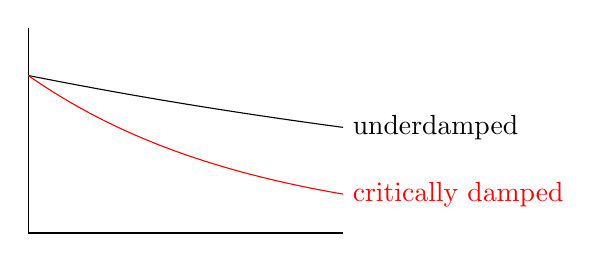
\begin{tikzpicture}[domain=0:2, samples=50, scale=2]
        \draw(0, 0) -- (2, 0);
        \draw(0, 0) -- (0, 1.3);
        \draw[color=black] plot (\x, {exp(-0.2* \x)}) node[right] {underdamped};
        \draw[color=red] plot (\x, {exp(-0.7 * \x)}) node[right] {critically damped};
    \end{tikzpicture}
\end{center}

Both of these curves are exponential decay curves, but the critically damped one goes to zero much faster than any other damping.

\section{Driving Forces}

Now imagine instead of a resistive force, that we have a driven force instead. That is, our equation of motion now looks like this: 

\[ F = -kx - bx + F_0 \cos(\omega t)\] 

where $F_0 \cos(\omega t)$ denotes the driving force, with $\omega$ being the angular frequency of the driving force. Therefore, we have the differential equation:

\[ \ddot x + 2\beta x + \omega_0^2x = f_0 \cos(\omega t)\] 

where $f_0 = \frac{F_0}{m}$, and $\beta$ is defin in the same way as before. This differential equation has two solutions: 

\begin{itemize}
    \item A homogeneous solution $x_h(t)$, which solves the differential equation when the right hand side is 0. 
    \item A particular soluiton, $x_p(t)$, which solves the differential equation while replicating the right hand side. 
\end{itemize}

Then, if we can find these two solutions, then we can combine them together: 

\[ x(t) = x_h(t) + x_p(t)\] 

We already know $x_h(t)$ from the earlier section, so if we can find an $x_p(t)$, then we have the full solution to the problem. We've seen before that sines and cosines seem to work well with oscillations, so why not try the solution $x_p(t) = A\cos(\omega t - \delta)$. Plugging this in, we get: 

\begin{align*}
    -A\omega^2 \cos(\omega t - \delta) - 2\beta A \omega \sin (\omega t - \delta) + \omega_0^2 A \cos(\omega t - \delta) = f_0 \cos \omega t\\
    f_0 \cos (\omega t) - A(\omega_0^2 - \omega^2)\cos(\omega t - \delta) + 2\beta A \cos(\omega t - \delta) = 0
\end{align*}

Now we use the trigonometric identities:

\begin{align*}
    \cos(\alpha - \beta) &= \cos \alpha \cos \beta + \sin \alpha \sin \beta\\
    \sin(\alpha - \beta) &= \sin \alpha \cos \beta - \cos \alpha \sin \beta
\end{align*}
    
Doing so we get the equation:


\[ \left \{ f_0 - A\left[ (\omega_0^2 - \omega^2)\cos \delta + 2\omega \beta \sin \delta \right]\right \} \cos (\omega t) -  \left \{A\left[ (\omega_0^2 - \omega^2)\sin \delta - 2\omega \beta \cos(\omega t)\right] \right \} \sin(\omega t) = 0\] 

Since $\sin(\omega t)$ and $\cos(\omega t)$ are linearly independent functions, this euqation is only satisfied when both terms are zero. From the first term, we get:

\begin{align*}
    \tan \delta &= \frac{2\omega \beta}{\omega_0^2 - \omega^2} \\
    \therefore \delta &= \tan^{-1}\left(\frac{2\omega \beta}{\omega_0^2 - \omega^2}\right)
\end{align*}

Therefore, 

\[ \sin \delta = \frac{2\omega \beta}{\sqrt{(\omega_0^2 - \omega^2)^2 + 4\omega^2 \beta^2}} \phantom{aaa} \cos \delta = \frac{\omega_0^2 - \omega^2}{\sqrt{(\omega_0^2 - \omega^2)^2 + 4\omega^2 \beta^2}}\]

From the cosine term, we get: 

\begin{align*}
    A &= \frac{f_0}{(\omega_0^2 - \omega^2)\cos \delta + 2\omega \beta \sin \delta}\\
    &= \frac{f_0}{\sqrt{(\omega_0^2 - \omega^2) + 4\omega^2 \beta^2}}
\end{align*}

so now we finally have the particular solution: 

\[ x_p(t) = A\cos(\omega t - \delta) = \frac{f_0 \cos (\omega t - \delta)}{\sqrt{(\omega_0^2 - \omega^2) + 4\omega^2 \beta^2}}\]

So our general solution, (again $x(t) = x_h(t) + x_p(t)$) is

\[ x(t) = C_1e^{r_1t} + C_2e^{r_2t} + A\cos(\omega t - \delta)\] 

Note that for large time, the $x_h(t)$ terms die out, but the $x_p(t)$ terms don't, and dominate for large time $t \gg \frac 1 \beta$. In other words: 

\[ x(t \gg \frac{1}{\beta}) = x_p(t)\] 

\subsection{The phase difference}

Earlier we said that $\delta$ represents the phase differene between the action and the resulting motion: 

\[ \delta = \tan^{-1}\left(\frac{2\omega \beta}{\omega_0^2 - \omega^2}\right)\] 

For a fixed $\omega_0$, as $\omega$ increases from 0, we get that the phase increases from $\delta = 0$ to $\delta = \pi/2$ at $\omega = \omega_0$ and $\delta \to \pi$ as $\omega \to \infty$.

\subsection{Amplitude} 

At large times, it's useful to look at the effect of $\omega$ on the amplitude by looking at $x_p(t)$. To find where $A$ is maximized, we simply take $\frac{dA}{d\omega} = 0$, giving us $\omega_2 = \sqrt{\omega_0^2 - 2\beta^2}$, so the resonance frequency is lowered as damping $\beta$ is increased. This makes sense intuitively, since the larger value of $\beta$ means that our oscillation decays much faster. 

\begin{insight*}{}{}
    Note that we don't get any resonance frequencies for $\beta^2 > \omega_0^2/2$, since that's when the square root becomes complex-valued.
\end{insight*}

[INSERT TIKZ HERE]

\section{Summary} 

In summary, so far we've looked at free, damped and driven oscillations: 
\begin{itemize}
    \item Free oscillations: $\omega_0 = \frac{k}{m}$
    \item Damped oscillations: $\omega_1 = \omega_0^2 - \beta^2$
    \item Driven oscillations: $\omega_2 = \omega_0 - 2\beta^2$
\end{itemize}

This set of relations gives us $\omega_0 > \omega_1 > \omega_2$. The maximum amplitude is given by 

\[ A_{max} = \frac{f_0}{\sqrt{4\omega^2\beta^2}} = \frac{f_0}{2\omega \beta}\]

This equation tells us that if we make $\beta$ smaller, then $A_{max}$ increases and also becomes taller and narrower. We define the \textit{full width half maximum} ($\text{FWHM} = 2\beta$ ) to quanitfy this value. 

\subsection{Aside: Quality Factor} 

We sometimes define a quality factor $Q$ as the ration of the resonance position $\omega_0$ to its width $2\beta$:

\[ Q = \frac{\omega_0}{2\beta}\] 

This means that large values of $Q$ correspond to narrow resonance, and small values correspond to a wide resonance. 

\section{Application: LC Circuits}

We've learned in electricity and magnetism (and also 5BL) that a simple LC circuit also behaves like an oscillator, since it follows the equation: 

\[ L \frac{dI}{dt} + \frac 1c \int I \ dt = 0\] 

or in terms of the charge $q$: 

\[ L \ddot q + \frac{1}{c} q = 0\] 

The solutions are of the same form since the only thing we've changed here are the variable names: $q(t) = q_0 \cos(\omega t)$. Overall, we can just perform the substtution of letters: 

\[ m \to L \phantom{aa} x \to q \phantom{aa} \frac 1k \to c \phantom{aa} \dot x \to I\] 

Similarly, adding a resistance will give us the equivalent of a damping term, and adding an AC power generator is the same as adding a driving force to the system. Again, the nature of these system is the exact same as what we just solved for, so the equations of motion remain the same as well.





%%%%%%%%%%%%%%%%%%%%%%%%%%%%%%%%%%%%%%%%%%%%%%LECTURE 3%%%%%%%%%%%%%%%%%%%%%%%%%%%%%%%%%%%%%%%%%%%%%%%%%%%%%%%%
    \chapter{Lecture 3 (8/29)}
    The third lecture of Physics 137A was held on  \textbf{Monday, August 29}. It discussed the wave description of matter and made a brief introduction to operators.

      \section{Last Time: Everything is a Wave (in Quantum Mechanics)}
          Last lecture we found that everything is a wave in Quantum Mechanics. This is true, but depending on the unit scales that we're talking about, the true wave descriptions of matter may not show. For instance: \

          \begin{itemize}
              \item Electrons: $\lambda_{dB} = e^{-1} \text{nm}$, atom size: 1 \AA. These sizes are comparable.
              \item Humans: $\lambda_{dB} = 10^{-36} \text{nm}$, size: ~1m. These sizes are nowhere near comparable
          \end{itemize}

          Since the size of everyday objects are so much larger than that of the deBroglie wavelength, this is why we don't see any quantum effects with the naked eye.

          Now back to the quantum realm. Because we've said already that everything is a wave, waves can also interfere with each other. Consider a wave source some distance away from a double slit. If we move the slit apparatus sufficiently far away from the source, the oncoming waves appear to be plane waves instead of circular (or spherical) wave patterns. This is what we mean by plane waves - the fact that the source is infinitely far away from us. To describe this wave, we can measure its electric field, which can be done in the following way:

          \[ \vec E = \vec{E}_0e^{i(k \cdot r - \omega t + \varphi)}\]

          The way we should interpret this expression is as follows: $\vec{E_0}$ is a description of the maximum allowable electric field intensity at any point in time, and $e^{i(k \cdot r - \omega t + \varphi)}$ represents a phase, or in other words, how much of the maximum intensity we are seeing at any point in time. The term $k \cdot r$ represents the spatial component (oscillations per unit space), and $\omega t$ represents the temporal component (oscillations in time). The $\varphi$ represents some overall offset phase, which is determined usually by the system.

          \begin{insight*}{}{}
              Note that we use a complex exponential here because $|e^{ikx}|^2 = 1$, which is particularly useful when we want it to represent as a percentage of the maximum allowable amplitude.\\\\
              This convention, we believe, is the fundamental reason why complex numbers exist in quantum mechanics! Any appearance of complex numbers we see later on comes from this convention.
          \end{insight*}

          Back to the double slit experiment. Since there are two slits, there are two sources, call them $\vec{E_1}$ and $\vec{E_2}$. Therefore, $E_{tot} = \vec{E_1} + \vec{E_2} = \vec{E}_{01}e^{i\delta_1} + \vec{E}_{02}e^{i\delta_2}$. Here, the $\delta_i$ represents the spatial and temporal frequencies. Since the intensity scales with $|E|^2 = E \cdot E^\star$ where $E^\star$ represents the complex conjugate, this gives:

          \begin{align*}
              |E|^2 &= E_{01}^2 + E_{02}^2 + \vec{E}_{01}\vec{E}_{02}\left(e^{i(\delta_2 - \delta_1)} + e^{-i(\delta_2 - \delta_1)}\right)\\
              &= E_{01}^2 + E_{02}^2 + 2\vec{E}_{01}\cdot \vec{E}_{02}\cos(\delta_2 - \delta_1)
          \end{align*}

          Notice the order of operations here: we summed the two electric field components \textbf{before} squaring them. This is important, since had we squared them first, then we would have simply gotten $\vec E_{01}^2 + \vec E_{02}^2$, which does not exhibit any interference pattern.

      \section{Wave Description of Matter}
          So, as we see from the double slit experiment and from our previous discussions on quantum mechanics, particles in the classical sense don't really exist, and everything can be modeled as a wave. So, how do we do this? With the help of a newly-defined \textbf{wave function:}
          \begin{definition}{Wave Function}{}
              Typically denoted $\Psi$: a complex function of position and time.
          \end{definition}
          More specifically, $\Psi$ is an amplitude. However, it's not physical (in other words, we can't directly measure it). Despite this, similar to position and momentum in classical mechanics, this wave function contains all of the physical information needed to describe the system.

          \subsection{Probability Density}
              For a while, we had no idea what to do with $\Psi$ and how to make it describe life precisely because it offered no physical significance on its own. However, in 1926, Max Born found that, by taking the square of the modulus of this function, we are able to actually glean something physical from the wave function. This gives us another important concept, notably \textit{probability density}:
              \begin{definition}{Probability Density}{}
              $P(\vec{r},t) = |\Psi(\vec{r},t)|^2$: The probability per unit volume of finding a \say{particle} at $\vec{r},t$.
              \end{definition}
              As we can see, squaring the modulus gives us a real, physical interpretation and something we can actually work with. Furthermore, to normalize, we multiply by our volume, so the probability within a cube $d\vec{r}$ becomes:
              $$P(\vec{r},t)d\vec{r} = |\Psi(\vec{r},t)|^2d\vec{r}$$
              For generality, we write $d\vec{r}$ to refer to a volume irrespective of any coordinate system.

      \section{Wave Superposition}
          Now, a key insight in quantum mechanics (and one that carries over from classical mechanics) is that of superposition:
          \begin{theorem}{Superposition}{superposition}
              If $\Psi_1$ and $\Psi_2$ are two allowed waves/states (solutions to some wave equation), then $$\Psi = c_1\Psi_1 + c_2\Psi_2$$ is also allowed, where $c_1,c_2 \in \mathbb{C}$.
          \end{theorem}
          We allow the constants to be complex to not eliminate the interference we saw earlier with our double slit experiment.

      \section{Introducing Operators}
          Now, if we recall classical mechanics, knowing the position and momentum gives us everything we could ever want to know about the system [INSERT TIKZ HERE]. Now, what happens if we try to throw a plane wave into our model? [INSERT TIKZ] We immediately run into a problem: the wave is everywhere. This means that position and velocity are essentially meaningless quantities to us here. So, how do we reconcile this?

          \subsection{de Broglie Relations}
              Recalling the de Broglie relations that we learned in high school:
              \begin{theorem}{de Broglie Relations}{de broglie relations}
                  For a quantum-mechanical system:
                  \begin{align*}
                      E &= hf = \hbar \omega &&\hbar = \frac{h}{2\pi}\\
                      p &= \frac{h}{\lambda} = \hbar k && k = \frac{2\pi}{\lambda}
                  \end{align*}
              \end{theorem}
              This allows us to better understand our system, but we still need to take it one step further.

          \subsection{Enter the Operator}
              Consider first a 1D particle: [INSERT TIKZ]
              In this case, we write out our wave function and we get:
              $$\Psi = Ae^{i(kw - \omega(k)t)}$$
              All of our vectors turn into scalars. Rewriting this, we get:
              $$\Psi = Ae^{\frac{i(p_xx - E(p_x)t}{\hbar}}$$
              This is great and all, but we want information about the momentum and the energy, and they're stuck in the exponent. How do we get them? Easy: \underline{take the derivative (with respect to either)}:
              \begin{align*}
                  -i\hbar\frac{\partial}{\partial x}\Psi &= p_x\Psi\\
                  i\hbar\frac{\partial}{\partial t}\Psi &= E\Psi
              \end{align*}
              If we look at these equations, they look suspiciously like equations with eigenvalues and eigenvectors, so if we consider just the eigenvectors, we get our \fbox{momentum and energy operators}:
              \begin{definition}{Momentum and Energy Operators}
                  We define these operators as such:
                  \begin{align*}
                      \text{Momentum}&: -i\hbar\frac{\partial}{\partial x}\\
                      \text{Energy}&: i\hbar\frac{\partial}{\partial t}
                  \end{align*}
              \end{definition}
              Now, we have another crucial tool that we will use a lot.
          \subsection{Operators in 3 Dimensions}
              We can obviously then extend this to three dimensions, where we see that the operators become \underline{gradients}:
                \begin{align*}
                    i\hbar\frac{\partial}{\partial t}\Psi &= E\Psi\\
                    -i\hbar\vec{\nabla}\Psi &= \vec{p}\Psi &&\vec{\nabla} = \begin{pmatrix}\frac{\partial}{\partial x}\\\frac{\partial}{\partial y}\\\frac{\partial}{\partial z}\end{pmatrix}
                \end{align*}
                It's important here to now remember that we have vectors rather than scalars.
        \section{Probability Density and Normalization}
            We have all of these cool values, but we need to remember that these need to be normalized for us to deal with them, so we have the following important insight:
            \begin{insight*}{}{}
              $\fbox{$\int_{\text{all space}}|\Psi(\vec{r},t)|^2dr = 1$}$: The probability that the \say{particle} is somewhere in space is $1$.
            \end{insight*}
            We will use this insight a lot.

            \subsection{Plane Waves are Problematic}
                Here, though, we already run into an issue: if we throw our plane wave into this equation, we see that the integral goes to $\infty$, since the wave exists everywhere in space and time. So, plane waves are far too simplistic a description of life.
            \subsection{Wave Packets and Fourier Transforms}
                Since we can't use plane waves, we need a type of wave that is localized rather than everywhere-permeating, where we get the \textit{wave packet}: [INSERT TIKZ]
                Clearly, it's much more difficult to deal with, but we will learn how to work with them. How do we get wave packets? We get them by \underline{adding together many plane waves} (of different amplitudes and frequencies), with a method that is more commonly referred to as a \fbox{Fourier Transform}. We will learn about how to do this in the next lecture.
%%%%%%%%%%%%%%%%%%%%%%%%%%%%%%%%%%%%%%%%%%%%%%LECTURE 4%%%%%%%%%%%%%%%%%%%%%%%%%%%%%%%%%%%%%%%%%%%%%%%%%%%%%%%%
    \chapter{Lecture 4 (8/31)}
    The fourth lecture of Physics 137A was held on \textbf{Wednesday, August 31}. It covered wave packets and reviewed the mathematics of the Fourier transform.
\section{Last Time: Wave Description of Nature}
    Last lecture, we explained how everything in the world, in the context of quantum mechanics, can be described as a wave and by a wave function. We started with a standard plane wave, described by the expression $e^{i(kx - \omega t)}$, where $k$ is the spatial frequency and $\omega$ is the temporal frequency. [INSERT TIKZ] Furthermore, we were given the de Broglie relations, which describe the momentum and energy of such a wave:
    \begin{align*}
        p &= \hbar k &&k = \frac{2\pi}{\lambda}\\
        E &= \hbar\omega &&\omega = 2\pi f
    \end{align*}
    From this, we see that a large $k$ will imply more momentum, and a large $\omega$ will imply more energy.\\\\
    While this is all well and good, we found that a plane wave doesn't really help us in describing localized phenomena, since it exists everywhere in space and time and we need the integral over all of space to come out to $1$. And so, for this, we will need to understand \textit{wave packets}, and this is our goal today: \underline{move from plane waves to wave packets}.

\section{Wave Packets}
    We currently have a plane wave permeating all of space: [INSERT TIKZ]
    We saw that this plane wave $e^{i(k_1x - \omega t)}$ is pretty OK at describing the wave at the specific location of interest, but as soon as we move away from it, it becomes exceedingly unhelpful. So, our target is a localized wave packet:
    [INSERT TIKZ]
    How can we get this? Well, let's add some more plane waves to our initial one:
    [INSERT TIKZ]
    As we can see, we can kill a lot of the terms past our desired localized region with the proper choices of $k_n$, since the waves will interfere with each other there. So, after adding together a bunch of $e^{i(k_m - \omega t)}$ waves, we get something that's pretty darn close to what we want:
    [INSERT TIKZ]
    But, we can't just add these waves together blindly: some waves will. have more of an effect in the sum than others. Because of this, we need to properly weight them. How do we do this? Through \textit{amplitudes}! And so, our sum becomes something more like this:
    $$A_0e^{i(k_1x - \omega t)} + A_1e^{i(k_2x - \omega t)} + A_2e^{i(k_3x - \omega t)} + A_3e^{i(k_4x - \omega t)} + \dots$$
    This as some have already no-doubt guessed, is exactly the beginning of a \fbox{Fourier Transform}.

    %maybe put this subsection into an example environment?
    \subsection{1D Wave Packet}
        Let's apply this to our simple 1D wave packet. To do this, let's throw in $p$ and $E$, so that we can deal with a wave function. So, our wave will look like $e^{i\frac{p_xx - E(p_x)t}{\hbar}}$. Summing over many plane waves gives us our new expression for $\Psi$:
        $$\Psi(x,t) = \frac{1}{\sqrt{2\pi\hbar}}\int e^{i\frac{P_xx - Et}{\hbar}}\phi(p_x)dp_x$$
        Here, it's important to realize that we are \textbf{integrating over momentum, not space or time}! This is because we are considering snapshots in space and time, for which the momentum will be changing. In this expression, notice that $\phi(p_x)$ is the weight parameter, which plays the role of the amplitudes $A_m$ we saw in the first sum we attempted to construct. Finally, the coefficient in front of the integral is our normalization, since we only want to deal with normalized wave functions.\\\\
        Now, a small 137A gift: we are going to work through the math of the Fourier transform and review everything necessary to move forward with our study of quantum mechanics.

  \section{Review of Fourier Transforms}
      Here, we are going to cover all of the mathematics of the Fourier transform that is important for our purposes. We won't be delving into too much specific detail; for that, consult some other reading materials from other courses. Now, let's cover all of the pieces of the transform.

      \subsection{Discrete Fourier Transform}
        Starting with the simplest form, we have the discrete Fourier transform, which can model the behavior of a period function $f(x) = f(x+2\pi)$, with $x \in [-\pi,\pi]$, as an example. From this, we get our first equation for the transform:
        $$f(x) = \frac12 A_0 + \sum_{n=1}^{\infty}[A_n\cos(nx) + B_n\sin(nx)]$$
        Writing this down is no big deal, but the hard part is figuring out these coefficients $A_n$ and $B_n$. This would be akin to being told the ingredients of coffee and being asked to make a perfect latte: you need the proper proportions of ingredients, not just the ingredients themselves. How do we do this?
        \begin{example}{Finding Components of Vectors}{}
          Consider a vector $\vec{v} = a\hat{x} + b\hat{y} + c\hat{z}$. How can we find the coefficients $a$, $b$, and $c$? Easy: take the dot product:
          \begin{align*}
            a &= \vec{v}\dot\hat{x}\\
            b &= \vec{v}\dot\hat{y}\\
            c &= \vec{v}\dot\hat{z}
          \end{align*}
          We can now apply this to our situation.
        \end{example}
        As we can see, taking the dot product can give us the components, so why don't we try something similar? This time, instead of taking a dot product, we can integrate. Remember, we hace to pick our \say{basis vectors} accordingly and normalize the integral. Doing so and putting everything together gives us the full expression with all of the components for the discrete Fourier Transform:
        \newpage
        \begin{definition}{Fourier Transform: Discrete Case}{}
            Given periodic function $f(x) = f(x+2\pi)$ with $x \in [-\pi,\pi]$:
              \begin{align*}
                f(x) &= \frac12A_0 + \sum_{n=1}^{\infty}[A_n\cos(nx) + B_n\sin(nx)]\\
                A_n &= \frac{1}{\pi}\int f(x)\cos(nx)dx\\
                B_n &= \frac{1}{\pi}\int f(x)\sin(nx)dx
            \end{align*}
        \end{definition}
        That's it for the discrete Fourier transform. Now, let's write it in terms of exponents.

      \subsection{Discrete Case: Exponential Form}
        Having written out the Fourier transform in terms of $\sin$ and $\cos$, let's write it out in terms of exponents, since we will be dealing with functions of this form a lot more. Converting everything gives us the following expression:
        \begin{definition}{Fourier Transform: Discrete Case with Exponents}{}
          Given the same periodic function:
          \begin{align*}
            f(x) &= \frac{1}{\sqrt{2\pi}}\sum_{n=-\infty}^{\infty}C_ne^{inx}\\
            C_n &= \frac{1}{\sqrt{2\pi}}\int_{-\pi}^{\pi}f(x)e^{-inx}dx
          \end{align*}
        \end{definition}
        It's at this point where we need to introduce a new tool: the \textit{Kronecker delta}.

      \subsection{Kronecker Delta}
        For the future, we will define this new function, which looks like this:
        \begin{definition}{Kronecker Delta}{}
          Denoted $\delta_{mn}$: $\frac{1}{\sqrt{2\pi}}\int_{-\pi}^{\pi}e^{i(n-m)x}dx = \fbox{$\delta_{mn} = \begin{cases}1 & \text{if } m = n\\ 0 & \text{if } m \neq n\end{cases}$}$
        \end{definition}
        This Kronecker delta establishes \textit{orthonormality}, since we want our vectors to be orthonormal. With that, we have finished with discrete Fourier transforms, and we can move on to understand the generalized continuous case.

      \subsection{Continuous Fourier Transform}
        In the continuum limit, the sums will become integrals, so our expressions will look like this:
        \begin{definition}{Fourier Transform: Continuous Case}{}
          Given the same period function:
          $$f(x) = \frac{1}{\sqrt{2\pi}}\int_{0\infty}^{\infty}g(k)e^{ikx}dk$$
          Here, $g(k)$ is defined as the \textbf{Fourier transform} of $f(x)$.
        \end{definition}
        How do we find the transform $g(k)$? Well, we can then take the \textit{inverse Fourier transform}:
        \begin{definition}{Inverse Fourier Transform}{}
          Given $g(k)$:
          $$g(k) = \frac{1}{\sqrt{2\pi}}\int_{-\infty}^{\infty}f(x)e^{-ikx}dx$$
          Then, $f$ is defined as the \textbf{inverse Fourier transform} of $g(k)$.
        \end{definition}
        These integrals we just saw are commonly referred to as \textbf{Fourier integrals}, and we will later learn that these are a special case of a \textit{unitary transform}.\\\\
        Similarly, we need to understand how the Kronecker delta behaves in the continuum limit.

      \subsection{Dirac Delta}
        As was probably surmised, in the continuum limit, the Kronecker delta becomes the much-feared \textit{Dirac delta function}. Let's expand out our integral to see where it comes from:
        $$f(x) = \frac{1}{2\pi}\int_{-\infty}^{\infty}\left[\int_{-\infty}^{\infty}f(x')e^{-ikx'}dx'\right]e^{ikx}dk$$
        Manipulating this:
        $$g = \int_{-\infty}^{\infty}f(x')\delta(x-x')dx$$
        And so, we get our Dirac delta function:
        \begin{definition}{Dirac Delta}{}
          Denoted $\delta(x-x')$: $\delta(x-x') = \frac{1}{2\pi}\int_{\infty}^{\infty}e^{ik(x-x')}dx$
        \end{definition}
        Now, this function is very odd and has some pretty weird properties, so let's explore them a bit here.\\\\
        Since $f(x)$ and $f(x')$ are arbitrary and independent, $\delta(x-x')$ must be $0$ if $x\neq x'$, and $\int \delta = 1$ otherwise. These properties need to hold in order for our integral to not fall apart, but these are still difficult to understand. To better comprehend just how a delta function behaves, let's illustrate this with a diagram:
          [INSERT TIKZ with descriptions]
        Here, we see that $g(k)$ must be infinitely sharp at exactly one point: $k_0$. Similarly, this implies that the Fourier transform for a single plane wave will be precisely the $\delta$ function. What happens if we add more waves?
          [INSERT TIKZ]
        As we can see, the function gains width, and decreases in sharpness. This will lead us nicely into the Uncertainty Principle later on.\\\\
        This marks the end of the mathematical review. Back to physics!

    \section{Back to Wave Packets}
      Recall our 1D wave packet: $$\Psi(x,t) = \frac{1}{\sqrt{2\pi\hbar}}\int_{-\infty}^{\infty}e^{i\frac{p_xx - E(p_x)t}{\hbar}}\phi(p_x)dp_x$$
      Now that we have our mathematical tools in place, let's expand this. Suppose $\phi(p_x)$ is a sharp function, but not quite as sharp as a delta function:
        [INSERT YET ANOTHER TIKZ]
      As we can see, the added width at the bottom will correspond precisely to increased uncertainty in the measurement of $p_x$.

      \subsection{Stationary Phase Condition}
        For added simplicity, let $\beta{p_x} = p_xx - E(p_x)t$. Then, our equation simplifies:
        $$\Psi(x,t) = \frac{1}{\sqrt{2\pi}}\int_{-\infty}^{\infty}e^{i\frac{\beta(p_x)}{\hbar}}\phi(p_x)dp_x$$
        Now, let's release the inner mathematician and try to see what is going on. If $\beta(p_x)$ varies, then the exponential component will rapidly oscillate. And, outside $p_0$, the weight $\phi(p_x)$ goes to $0$. The oscillation in the exponent will disappear when $\beta$ goes to $0$. This is referred to as the \textbf{stationary phase condition}. Let's try to look for it.

      \subsection{Group Velocity}
        The stationary phase condition, by definition, will be an inflection point, so we need to set the derivative to $0$:
        $$\frac{d\beta(p_x)}{dp_x}\Biggr|_{p_x = p_0} = 0$$
        Computing this gives:
        $$x - \left(\frac{d}{dp_x}E(p_x)\right)t = 0 \implies \frac{x}{t} = \frac{dE(p_x)}{dp_x}\Biggr|_{p_{x=0}}$$
        Many will recognize that last expression as the \textit{group velocity}:
        \begin{definition}{Group Velocity}{}
          Denoted $v_g$: $$v_g = \frac{dE(p_x)}{dp_x}\Biggr|_{p_{x=0}}$$
          Group velocity refers to \textbf{how fast the center of the wave packet moves}.
        \end{definition}
        Even though all of the individual waves will most likely be traveling at different speeds, the whole wave packet group will travel at one velocity, which we just derived.

      \subsection{Phase Velocity}
        Now, if group velocity is the velocity of the group wave packet, then we also want to find the velocity of any individual wave. To do this, we can find the stationary phase condition for an individual plane wave:
        \begin{align*}
          e^{i(k_0x - \omega(k_0)t)}\\
          \therefore k_0x - \omega(k_0)t &= 0 &&\text{(set phase to $0$ for SPC)}\\
          \therefore \frac{x}{t} \frac{\omega(k_0)}{k_0} = \frac{E(p_0)}{p_0}
        \end{align*}
        That last expression is precisely our phase velocity:
        \begin{definition}{Phase Velocity}{}
          Denoted $v_p$: $$v_p = \frac{\omega(k_0)}{k_0} = \frac{E(p_0)}{p_0}$$
          The phase velocity refers to \textbf{how fast any individual plane wave is traveling}.
        \end{definition}
        It'll be super crucial to remember the difference between these two different velocity types!

    \section{Next Time: Dispersion}
      Now, because of these differences between phase and group velocity, we actually find that, with time, the wave packets will \textit{disperse}. We will build on this next time.
%%%%%%%%%%%%%%%%%%%%%%%%%%%%%%%%%%%%%%%%%%%%%%LECTURE 5%%%%%%%%%%%%%%%%%%%%%%%%%%%%%%%%%%%%%%%%%%%%%%%%%%%%%%%%
            \chapter{Lecture 5 (9/2)}
              The fifth lecture of Physics 137A was held on \textbf{Friday, September 2}. It covered more on wave packets and built up to the Heisenberg uncertainty principle.

              \section{Last Time: Wave Description of Matter for Free Particle}
                From the previous lectures, we want a wavelike description of matter. To accomplish this, we've been playing around with the free particle [INSERT TIKZ] Modeled as a wave, this becomes a wave packet described by the wave function $\Psi(x)$, where $|\Psi(x)|^2$ is the probability density to find the \say{particle} at $x$. [INSERT TIKZ] Note that this \underline{isn't a plane wave}: plane waves go on forever and we want to localize our wave function just where the \say{particle} is. Despite this, plane waves are just fine for some approximations in the right regions:
                \begin{example}{Wave Between two Walls}{}
                    Here, we have two different functions between two walls. As we can see, for this small approximation, the wave packet and the plane wave are basically the same, so a plane wave (which is much simpler to model) suffices as a decent approximation.
                \end{example}
                With all of this, we constructed a formula for our wave function:
                $$\Psi(x) = \frac{1}{\sqrt{2\pi\hbar}}\int_{-\infty}^{\infty}\exp{i\frac{p_xX - E(p_x)t}{\hbar}}\phi(p_x)dp_x$$
                As we found, writing out this equation is easy, but the hard part is figuring out the weight $\phi$, which we can do with the Fourier transform, a trick which we learned last time.

                \subsection{Modeling $\mathbf{\phi}$}
                  As we found, for a single plane wave, $\phi(p_x)$ is a delta function at $p_0$ [INSERT TIKZ] Adding more plane waves gives us a delta function that spreads out. This is our \textbf{first level of approximation}.

                \subsection{Uncertainties Everywhere}
                  From that model, we can see the following key insight which will become important later on:
                  \begin{insight*}{}{}
                    Having no uncertainty in momentum gives no information for position, and having no uncertainty in position gives no information for momentum
                  \end{insight*}
                  This will come up later when we develop the Heisenberg uncertainty principle. Similarly, we had another insight when calculating the phase velocities $v_p$ and group velocity $v_g$ of our wave packet:
                  \begin{insight*}{}{}
                    Because each plane wave in the wave packet has a different momentum (and by extension phase velocity, the wave packet will eventually \underline{disperse.}
                  \end{insight*}
                  With all of these tools, let's continue playing around with the free particle.

            \section{Playing Around with our Function}
              Consider some distribution for $\phi$ which is not quite a delta function: [INSERT TIKZ]
              Recalling our equations for group velocity, we have $$v_g = \frac{\partial \omega}{\partial k} = \frac{\partial E}{\partial p}$$
              Since we're modeling a particle here, the classical velocity $v$ exactly corresponds to the group velocity $v_g$: $$v = v_g = \frac{p_x}{m}$$
              So, $\frac{\partial E(p_x)}{\partial p_x} = \frac{p_x}{m}$, which means that $$E(p_x) = \frac{p_x^2}{2m}$$
              This is the exact formula for kinetic energy that we expect in classical mechanics!

              \subsection{Energy for Plane Wave}
                In the case of a single plane wave, that means that $$E(p_x) = \frac{p_0^2}{2m}$$
                How can we add more terms to this to get an expression for an actual wave packet that isn't just a delta function? \textit{Taylor expand}!

              \subsection{Energy for Wave Packet}
                Taylor expanding our equation gives us:
                $$E(p_x) = \frac{p_0^2}{2m} + \frac{p_0}{m}(p_x-p_0) + \frac{(p_x - p_0)^2}{2m}$$
                Note that these are the only three terms in the Taylor expansion since the derivative is with respect to $p_0$. Now, plugging this into our wave function:
                $$\Psi(x,t) = \frac{1}{\sqrt{2\pi\hbar}}\int_{-\infty}^{\infty}\exp{i\frac{p_xx - (E(p_0)t + v_gt(p_x-p_0 + \frac{(p_x-p_0)^2}{2m}t}{\hbar}}\phi(p_x)dp_x$$
                Note that $v_g$ is simply $\frac{p_0}{m}$. Now, there are a lot of term corrections here, so how can we drop that ugly second-order correction? Well, we can drop it when $\frac{(p_x-p_0)^2t}{2m\hbar} \ll 1$. This actually gives us something important:
                \begin{insight*}{}{}
                  The second-order correction term gives you information about the dispersion time for the wave packet: for small $t$, the packet won't disperse, but for a sufficiently large $t$, the packet will spread out.
                \end{insight*}
                Coming back to our wave function:
                $$\Psi(x,t) = \frac{1}{\sqrt{2\pi\hbar}}\int_{-\infty}^{\infty}\exp{i\frac{p_xx - E(p_0)t - v_gt(p_x-p_0)}{\hbar}}\phi(p_x)dp_x$$
                This is quite a clunky expression. How do we make progress on solving this?

              \subsection{Adding $\mathbf{1}$ or Multiplying by $\mathbf{0}$}
                One very useful trick that came up a lot in algebra and will make a stunning reappearance here in physics is the trick of \textbf{multiplying by $1$ or adding $0$}. In other words, if we add a nice-looking expression that neatly fixes our equation while not actually changing the result, we can have a much easier time. So, let's try adding (and subtracting) $p_0x$:
                $$\Psi(x,t) = \frac{1}{\sqrt{2\pi\hbar}}\int_{-\infty}^{\infty}\exp{i\frac{p_xx - p_0x + p_0x - E(p_0)t - v_gtp_x + v_gtp_0}{\hbar}}\phi(p_x)dp_x$$
                Now pull out all of the constant terms with respect to $dp_x$:
                $$\Psi(x,t) = \frac{1}{\sqrt{2\pi\hbar}}e^{i\frac{p_0x - E(p_0)t}{\hbar}}\int_{-\infty}^{\infty}\exp{i\frac{(p_x-p_0)(x-v_gt)}{\hbar}}\phi(p_x)dp_x$$
                Notice that we ended up with a plane wave as one of the factors in the front! Similarly, we have thrown all information about our envelope in the exponential! Let's call the new expression in our integral $$\exp{i\frac{(p_x-p_0)(x-v_gt)}{\hbar}}\phi(p_x) = \fbox{$F(x,t)$}$$
                Notice what this is:
                %could either be theorem or definition as well
                \begin{insight*}{}{}
                  The function
                  $$\Psi(x,t) = \frac{1}{\sqrt{2\pi\hbar}}\exp{i\frac{p_0x_0 E(p_0)t}{\hbar}}\int_{-\infty}^{\infty}F(x,t)dp_x$$
                  is a \textbf{plane wave modulated by envelope $F$, moving at speed $v_g$}.
                \end{insight*}
                Calculating the probability density gives us:
                $$|\Psi(x,t)|^2 = |F(x,t)|^2$$
                The rest has modulus $1$, so it disappears.\\\\
                Now, let's model our distribution. As we can clearly see with the previous graphs for the distribution of $\phi$, the distribution of $\Psi$ will look like a \underline{Gaussian}!

          \section{Gaussian Wave Packets}
            As we've discussed before, approximations are key in physics. So, looking at our distribution for $\phi$, we see that the best model for it would be that of a Gaussian:[INSERT TIKZ]
            A Gaussian distribution is then defined as such:
            \begin{definition}{Gaussian Distribution}{}
              A distribution of the form $$f(x) = \frac{1}{\sigma\sqrt{2\pi}}\exp{-\frac12\left[\frac{x - \mu}{\sigma}\right]^2}$$
            \end{definition}
            In our case, our $\phi$ then looks like this:
            $$\phi(p_x) = C\exp{-\frac{(p_x-p_0)^2}{2(\Delta p_x)^2}}$$
            So, $|\phi|^2$ falls to $\frac{1}{e}$ for $p_x = p_0 \pm \Delta p_x$.

            \subsection{Computing $\mathbf{\Psi}$}
              To proceed, we're going to introduce an important identity from mathematics that we will assume to be given:
              \begin{theorem}{Integral Identity}{}
                $$\int_{-\infty}^{\infty}e^{-\alpha u^2}e^{-\beta u}du = \left(\frac{\pi}{\alpha}\right)^{\frac12}e^{\frac{\beta^2}{4\alpha}}$$
              \end{theorem}
              We could prove this with complex analysis, but we'll just take it to be true. Now, let's go back to $\Phi(x,t)$, but take a snapshot at $t=0$. Essentially, we are eliminating time dependence here (though on the homework we will re-introduce time dependence to get a full picture of our wave function). With $t=0$, we can eliminate everything that has a factor of $t$ in it from our expression. This then gives us:
              $$\Psi(x) = \frac{1}{\sqrt{2\pi\hbar}}\int_{-\infty}^{\infty}e^{i\frac{p_xx}{\hbar}}\phi(p_x)dp_x$$
              As we can see, in the time-independent case, this is a true Fourier transform of $\phi(p_x)$. As stated before, on the homework, we will put back $t$ to find the full expression for $\Psi$.\\\\
              How do we solve this? Just plug it into our identity! Plugging in, we get:
              $$\Psi(x) = \frac{1}{\sqrt{2\pi\hbar}}C\int \exp{i\frac{p_xx}{\hbar}}\exp{-\frac{(p_x-p_0)^2}{2(\Delta p_x)^2}}dp_x = \frac{\pi^{-\frac14}}{\sqrt{\alpha}}(\Delta p_x)^{\frac12}\exp{i\frac{p_0x}{\hbar}}\exp{-\frac{(\Delta p_x)^2x^2}{2\hbar^2}}$$
              As we can see, this last term is yet another Gaussian! This confirms an important fact:
              \begin{insight*}{}{}
                The Fourier transform of a Gaussian is also a Gaussian.
              \end{insight*}

            \subsection{Arriving at the Heisenberg Uncertainty Principle}
              In other words, this means that \fbox{$\Psi(x)$ looks like a Gaussian}: [INSERT TIKZ] This time, $\Psi$ falls to $\frac{1}{e}$ of the maximum at $x = \pm \Delta x$. Rewriting this, we have another crucial identity:
              \begin{theorem}{Heisenberg Uncertainty Principle: Equivalence Case}{}
                $$\Delta x = \frac{\hbar}{\Delta p_x}$$
              \end{theorem}
                This is the famed Heisenberg Uncertainty Principle that we were searching for! Notice that for a Gaussian wave packet, it's an equality. This is the \textit{minimum amount of uncertainty}. Every other wave packet will have a bigger uncertainty. We may prove this later, but it's hard. And so, we have that the Gaussian wave packet is the \underline{minimum uncertainty state}:
                \begin{definition}{Minimum Uncertainty State}{}
                  The state where uncertainty is minimized (as name suggests).
                \end{definition}
                So, for a non-Gaussian wave function, we can rewrite this principle into a form we all know and love:
                \begin{theorem}{True Heisenberg Uncertainty Principle}{}
                  $$\Delta p_x\Delta x \geq \hbar$$
                \end{theorem}

          \section{Heisenberg Uncertainty Principle: What does it Mean?}
            And so, we have calculated the space part of our wave function, and we will calculate the time part on the homework. Now, before we can move on with the rest of quantum mechanics, it is important for us to answer this question completely and correctly: \textit{what does the Heisenberg uncertainty principle mean?} Trying to unpack the inequality gives us this insight into the meaning of this simple expression:
            \begin{insight*}{}{}
                If you measure $\Psi(x)$ and measure it to an accuracy of $\Delta x = a$, then that means that immediately measuring $p$ will have some uncertainty $\Delta p$ which must be larger than equal to $\frac{\hbar}{\Delta x}$.
            \end{insight*}
            Notice the simultaneity condition for these measurements: the wave function will change with time, so this doesn't necessarily have to hold if one were to wait some amount of time before taking the measurement for $p$. But, in our case, where we are still dealing with instantaneous measurements, then this will hold.
            \newpage
            \subsection{Proving the Heisenberg Uncertainty Principle}
              How did Heisenberg prove his principle? With the help of a special tool: the \textit{Heisenberg microscope}:
              %could take this out of example environment if you so desire
              \begin{example}{Heisenberg Microscope}{}
                The following is a model for the microscope: [INSERT TIKZ] As we can see, we have an emitter passing electrons one at a time through a double slit. As we know from wave mechanics, this will produce an interference pattern on the back panel. However, we want to see inside of this, so we must illuminate the box with some gamma rays of wavelength $\lambda_{\gamma}$. This will then deflect the path of some of the electrons by some error $\Delta p_{e^{-1}}$ and some angle $\Delta \theta$. Now, if we want to resolve which slit a given electron came from, we must have that $$\lambda_{\gamma} < d$$
                Now, from our de Broglie relations, $p_{\gamma} = \frac{h}{\lambda_{\gamma}}$. Plugging this in, we have the following:
                \begin{align*}
                  \Delta p_{e^{-1}} \approx \frac{h}{\lambda_{\gamma}} &\geq \frac{h}{d}\\
                  \therefore d\Delta p_{e^{-1}} &\geq h\\
                  \therefore \Delta \theta \approx \frac{\Delta p_{e^{-1}}}{p_{e^{-1}}} &= \frac{h}{pd} = \frac{\lambda_e}{d}\\
                  \therefore L\Delta \theta = \lambda_{e^{-1}}\frac{L}{d}
                \end{align*}
              \end{example}
              The takeaway here is that \underline{trying to measure the momentum loses the interference pattern}. And so, this uncertainty principle must hold.

%%%%%%%%%%%%%%%%%%%%%%%%%%%%%%%%%%%%%%%%%%%%%%LECTURE 6%%%%%%%%%%%%%%%%%%%%%%%%%%%%%%%%%%%%%%%%%%%%%%%%%%%%%%%%
      \chapter{Lecture 6 (9/7)}
        The sixth lecture of Physics 137A was held on \textbf{Wednesday, September 7}. It covered a final review on wave packets and introduced the Schrodinger equation and Hermiticity.

        \section{Last Time: Waves and Wave Packets}
          What have we learned so far? So far, we have learned that everything is a wave. Why do we say this? We say it, because a wave description of matter is a more accurate and all-encompassing description than our previous particle model. Case in point: the double slit experiment. That experiment seems to definitively confirm that waves are the best description. Now, we had two different types of waves that we could use: plane waves and wave packets.\\\\
          Plane waves are everywhere, meaning that they are merely an approximation. While they're bad over large intervals, they are pretty decent over certain intervals.\\\\
          Secondly, wave packets are localized collections of many plane waves. Specifically, we have been considering wave packets that are localized in \textbf{space} and \textbf{momentum}. Then, the Heisenberg uncertainty principle gave us that
          $$\Delta p_x\Delta x \geq \hbar$$
          Heisenberg illustrated this principle with the \textit{Heisenberg microscope} thought experiment, explored last time.

        \section{Localization in Energy and Time}
          We explored localization in space and momentum, but we could also think about a wave packet being localized in \textbf{frequency} and \textbf{time}. In other words, we can think of it as a snapshot in time.
          \subsection{Another Uncertainty Relation}
            Now, with what we discovered, we see that, should our wave packet be localized in time and frequency, this means that we need another uncertainty relation for these two quantities. And so, we have the following:
            \begin{theorem}{Uncertainty Relationship for Time}{}
              $$\Delta E \Delta t \geq \hbar$$
              We write it this way, because $E = \hbar\omega$
            \end{theorem}
            Now, this relationship does look nice, but how can we confirm that it's actually accurate? Well, let's see why this works.
          \subsection{Model of the Atom}
            Now, we're going to illustrate why our uncertainty principle works:
            \begin{example}{Bohr Atom}{}
              Consider a simplified model of the standard Bohr atom:
              [INSERT TIKZ]
              Here, the electron has two possible states: a \textbf{ground state} and an \textbf{excited state}. The electron can reside in the ground state for as long as it desires, because there is no lower energy state for it to drop down to. However, when it's in the excited state, it will have some decay half-life. What do we mean by this? Well, at any given moment, the electron has some chance of dropping down to the ground state, and averaging out over a long time gives us a general curve which can help us predict after what time we can expect there to be a roughly 50\% chance that the electron has decayed into the lower state.\\\\
              Can we predict when this decay will happen? No, quantum mechanics won't let us. But we can average to get some half-lifetime $\tau$.\\\\
              Now, if we consider the uncertainty in the energy, we see that the higher energy level will actually have some width to it (since we don't actually know the exact energy), and this uncertainty will be equal to $\Delta E = \frac{\hbar}{\tau}$. \\\\
              In the ground state, the decay time is essentially infinite, so the uncertainty in the energy is practically negligible. However, in the excited state, we will have some decay time $\tau_{e}$, with a corresponding uncertainty in the excited energy $\Delta E_e = \frac{\hbar}{\tau_e}$. In other words, the emission will have some width:
              [INSERT TIKZ]
            \end{example}
            Now, let's take it a bit further and examine some more details about this uncertainty, specifically with what happens when an electron does jump down to a lower energy state:
            \begin{example}{Fluorescent Lights}{}
              Consider some fluorescent tube: [INSERT TIKZ]
              How does it work? Well, the edges are blasted with some electricity, and the gas inside heats up and glows a specific light frequency as a plasma. But why does the whole tube light up when just the edges are excited?\\\\
              Well, when electrons jump to lower states, they release photons. So, when the atom releases a photon, Newton tells us that the atom must have some recoil in the opposite direction: [INSERT TIKZ] But still, how can the next atom in the chain absorb emitted light coming from a different atom if it ends up recoiling? Because the recoil is small compared to the line width! This means that we get \textit{resonant absorption}.\\\\
              Notice that this doesn't apply for nuclei or gamma rays, since the line width then becomes small compared to the recoil. There is actually one case when the nuclei can absorb: \underline{when the entire lattice recoils.} [INSERT TIKZ]
              When the lattice recoils, the recoil will then be distributed over many particles in the lattice, and so the recoil will once again fall into the limit of being shorter than the line width, hence resonant absorption.\\\\
              This is actually the famous \textbf{M\"{o}ssbauer Effect}!
            \end{example}
            With that, we're done with waves and wave packets. Now it's time to move on to the \schrodinger equation.

          \section{The Schrodinger Equation}
            Now, we can move on to understanding one of the most important equations in not just quantum mechanics, but in physics as a whole.

            \subsection{How do We Find Wave Functions?}
              We have good expressions for the wave function, but our biggest problem right now is actually finding this wave function. We've been told what it is and what it looks like, but we can't actually find it for some given parameters. We need something akin to Newton's Second Law of Motion, but just for waves.

            \subsection{Equations for Wave-Equation for Quantum Mechanics}
              This wave equation must satisfy a few important conditions:
              \begin{itemize}
                \item{Linear (permits superposition): waves can be added}
                \item{Should reproduce (\say{agree} with) classical physics}
                \item{Boundary conditions}
              \end{itemize}
              To review what these mean, we firstly want to be able to add waves with our equation, which means it must be linear. Secondly, we don't want any previously-established laws of physics to break with this new equation, so the other laws must still be satisfied. Finally, our equation must satisfy some important boundary conditions. Let's look at those a bit more in-depth here.\\\\
              The classical wave equation has two derivatives in space and two derivatives in time. This means that we must impose two boundary conditions for us to get some kind of expression. However, this is bad news for us, because classically, we only need one boundary condition in order to invoke Newton's Second Law. So, our new wave equation should only have \textit{one time derivative to satisfy causality}.\\\\
              Let's now construct this wave equation!

            \subsection{\schrodinger Equation: the 1D Free Particle Case}
              Firstly, let's consider the system we've been trying to understand for a while: a free particle in one dimension. [INSERT TIKZ] So, this system is then described by a wave function $$\Psi(x,t) = Ae^{i\frac{p_xx - Et}{\hbar}}$$
              Now, recall ten that we can write energy as
              $$E = \frac{p_x^2}{2m}$$
              Substituting some expressions into the terms gives us our dispersion relation:
              $$\fbox{$\omega = \frac{\hbar k^2}{2m}$}$$
              Now, remember operators? We had the following note before:
              $$\frac{\partial \Psi(x,t)}{\partial t} = A(-i\omega)e^{i(kx-\omega t)} = -i\omega\Psi = -\frac{i}{\hbar}E\Psi$$
              Taking two derivatives in space, we similarly get:
              $$\frac{\partial^2}{\partial x^2}\Psi(x,t) = -k^2Ae^{i(kx-\omega t)} = -\frac{p_x^2}{\hbar}\Psi = -\frac{2Em}{\hbar^2}\Psi$$
              We have two $E$s, so let's group the equations together and solve to get this very crucial equation:
              \begin{theorem}{\schrodinger Equation for Free Particle in 1 Dimension}{}
                $$\fbox{$i\hbar\frac{\partial}{\partial t}\Psi(x,t) = \frac{\hbar^2}{2m}\frac{\partial^2}{\partial x^2}\Psi(x,t)$}$$
              \end{theorem}
              Now, if we think of those original terms in front of the $\Psi$s as operators, we have our momentum and energy operators as before:
              $$\hat{E} = i\hbar\frac{\partial}{\partial t}, \hat{p}_x = -i\hbar\frac{\partial}{\partial x}$$
              But, this is only for a free particle in one dimension, so we have to add in potential energy and the other dimensions. More correctly, we need to take into account a force that can be derived from a potential.

            \subsection{Correcting the Equation}
              What types of forces can be derived from a potential? \textbf{Conservative forces}! They then are described as the gradient of some potential:
              \begin{definition}{Conservative Force}{}
                Recalling from mechanics, this refers to a force that can be derived from a potential, which makes work done independent of a path.
              \end{definition}
              So, consider some conservative force:
              $$\vec{F}(\vec{r},t) = -\vec{\nabla}V(\vec{r},t)$$
              Here, $V$ is our potential. Writing this out in terms of operators, we have:
              \begin{definition}{Potential Operator}{}
                $$\hat{V}(\vec{r},t)\Psi(\vec{r},t) = V(\vec{r},t)\Psi(\vec{r},t)$$
                Here, $\hat{V}$ is our \textbf{potential operator}.
              \end{definition}
              Throwing this all together, we get:
              \begin{theorem}{\schrodinger Equation}{}
                $$\fbox{$i\hbar\frac{\partial}{\partial t}\Psi(\vec{r},t) = \left[-\frac{\hbar^2}{2m}\nabla^2 + \hat{V}(\vec{r},t)\right]\Psi(\vec{r},t)$}$$
              \end{theorem}
              This is exactly the equation that Erwin \schrodinger wrote down in 1926. This equation is super important, and you should remember it for the rest of your life.
              \begin{insight*}{}{}
                Notice that the first term in the brackets of the equation corresponds exactly to the \textbf{kinetic energy} component, whilst the second term in the bracket sum is the \textbf{potential}. Finally, the entire expression in the bracket is exactly the \textbf{Hamiltonian Operator} $\hat{H}$.
              \end{insight*}
              \begin{definition}{Hamiltonian Operator}{}
                Denoted $\hat{H}$: $\hat{H} = -\frac{\hbar^2}{2m}\nabla^2 + \hat{V}(\vec{r},t)$
              \end{definition}
              In other words, at its most basic, the \schrodinger equation is simply an equation of \underline{energy conservation}. Let's now talk about some properties of these operators.

          \section{Properties of $\Psi$, $\hat{H}$}
            Firstly, we have our most important property: probability conservation:
            $$\int_{\text{All Space}}|\Psi(\vec{r},t)|^2d\vec{r} = 1$$
            Now, let's derive \textit{hermiticity}. Taking the derivative here gives:
            $$\frac{\partial}{\partial t}\int_{\text{All Space}}|\Psi(\vec{r},t)|^2d\vec{r} = 0$$
            An important thing to remember here:
            \begin{insight*}{}{}
              Never listen to mathematicians! You can move derivatives anywhere! Everything is smooth. If it weren't, life would be discontinuous.
            \end{insight*}
            Notice that $|\Psi|^2$ is actually a different way of writing $\Psi^{*}\Psi$. So, throwing that in gives:
            $$\frac{\partial}{\partial t}\int_{\text{All Space}}|\Psi|^2d\vec{r} = \int_{\text{All Space}}\Psi^{*}\left(\frac{\partial \Psi}{\partial t}\right) + \int_{\text{All Space}}\left(\frac{\partial \Psi^{*}}{\partial t}\right)\Psi d\vec{r}$$
            Now, let's substitute in our operators:
            \begin{align*}
              i\hbar\frac{\partial}{\partial t}\Psi(\vec{r},t) &= \hat{H}\Psi(\vec{r},t)\\
              -i\hbar\frac{\partial}{\partial t}\Psi^{*}(\vec{r},t) &=\left[\hat{H}\Psi(\vec{r},t)\right]^{*}
            \end{align*}
            So, throwing this all in gives:
            \begin{align*}
              \int_{\text{All Space}}\Psi^{*}\left(\frac{\partial \Psi}{\partial t}\right) + \int_{\text{All Space}}\left(\frac{\partial \Psi^{*}}{\partial t}\right)\Psi d\vec{r} &= \frac{1}{i\hbar}\int_{\text{All Space}}\left[\Psi^{*}(\hat{H}\Psi) - (\hat{H}\Psi)^{*}\Psi\right]d\vec{r} = 0\\
              \therefore \int_{\text{All Space}}\Psi^{*}(\hat{H}\Psi)d\vec{r} &= \int_{\text{All Space}}(\hat{H}\Psi)^{*}\Psi d\vec{r} = \int_{\text{All Space}}\Psi^{*}\hat{H}^{*}\Psi d\vec{r}
            \end{align*}
            Since this integral we've been calculating is arbitrary for any surface, we have then:
            \begin{theorem}{Hermiticity}{}
              $$\hat{H} = \hat{H}^{*}$$
              Here, $\hat{H}$ has a special name:
              \begin{definition}{Hermitian Operator}{}
                Denoted $\hat{H}$.
              \end{definition}
            \end{theorem}
            And so, we have derived Hermiticity. This gives us this important fact:
            \begin{insight*}{}{}
              $E$ must be real number always.
            \end{insight*}
            We will continue with this and with expectation values next time.
        

%%%%%%%%%%%%%%%%%%%%%%%%%%%%%%%%%%%%%%%%%%%%%%LECTURE 7%%%%%%%%%%%%%%%%%%%%%%%%%%%%%%%%%%%%%%%%%%%%%%%%%%%%%%%%
      \chapter{Lecture 7 (9/9)}
        The seventh lecture of Physics 137A was held on \textbf{Friday, September 9}. It covered more on the \textbf{\schrodinger equation} and introduced \textbf{Hermiticity and the commutator}.

        \section{Last Time: \schrodinger Equation Describes Conservation of Energy}
            Last lecture, we tried to better understand the \schrodinger equation by modeling it as an equation that, like Newton's Second law with conservation of momentum, basically describes the conservation of energy for a wave function. We noted that total energy can be written as the sum of some kinetic energy $KE$ and some potential energy $PE$. These energy components were then defined by their separate operators, where total energy was described by the \textit{Hamiltonian operator} $\hat{H}\Psi = i\hbar\frac{\partial \Psi}{\partial t}$, kinetic energy was described by the \textit{momentum operator} $\frac{\hat{p}^2}{2m}\Psi = \left(-i\hbar\frac{\partial}{\partial x}\right)^2\Psi$, and finally the potential energy was described by a \textit{potential operator} $\hat{V}\Psi$. So, in the end, the equation became:
            $$i\hbar\frac{\partial \Psi}{\partial t} = \left[-\frac{\hbar^2}{2m}\frac{\partial^2}{\partial x^2} + \hat{V}(x)\right]\Psi = E\Psi$$
            Notice that the Hamiltonian and momentum operators are unique and will remain the same for all cases of the wave function $\Psi$. However, the potential operator $\hat{V}$ is not unique, so we will spend roughly a third of the course figuring out different cases for this operator.\\\\
            We also started on Hermiticity:
            \begin{align*}
                \int|\Psi(\vec{r},t)|^2d\vec{r} &= 1\\
                \therefore \frac{\partial}{\partial t}\int|\Psi(\vec{r},t)|^2d\vec{r} &= 0 = \int\Psi^{*}\left(\frac{\partial \Psi}{\partial t}\right) + \left(\frac{\partial \Psi^{*}}{\partial t}\right)\Psi d\vec{r}
            \end{align*}
            We need to generalize the $^{*}$ here, since it won't always be just the complex conjugate. But we need something new if we want to substitute \schrodinger into this. So, our generalization (from linear algebra) becomes the \underline{\textbf{adjoint}}. For scalars, it will remain the complex conjugate, but for matrices, it will be the conjugate transpose. We will, typically, use $^{\dagger}$ to denote the adjoing (a \say{dagger}).

        \section{Substituting in \schrodinger}
            Now, substituting in the \schrodinger equation:
            \begin{align}
                \frac{1}{i\hbar}\int\left[\Psi^{*}(\hat{H}\Psi) - (\hat{H}\Psi)^{*}\Psi\right]d\vec{r} \to \fbox{$\hat{H} = \hat{H}^{*}$} \label{eq1}
            \end{align}
            This gives us the Hermitian operator (the adjoing is equal to the normal).
            \begin{theorem}{Hermitian Operator Properties}{}
                The Hermitian operator is associated with two things:
                \begin{itemize}
                    \item{Real eigenvalues}
                    \item{Observables (needs to be a measurable quantity)}
                \end{itemize}
            \end{theorem}
            Now, let's do something with equation \ref{eq1}. Substitute the spatial part of the \schrodinger equation into equation \ref{eq1} (assume a real-valued $\hat{V}$):
            $$\dots = \frac{i\hbar}{2m}\int\left[\Psi^{*}(\nabla^2\Psi) - (\nabla^2\Psi^{*})\Psi\right]d\vec{r} = \dots$$
            Now, use the vector identity for the Laplacian: $\nabla^2 x = \vec{\nabla}\cdot\vec{\nabla}(x)$:
            $$\dots = \frac{i\hbar}{2m}\int\vec{\nabla}\cdot\left[\Psi^{*}(\vec{\nabla}\Psi) - (\vec{nabla}\Psi)^{*}\Psi\right]d\vec{r} = \dots$$
            Now, call the integrand $\vec{j}$:
            $$\dots = -\int\vec{\nabla}\cdot\vec{j}d\vec{r}$$
            Use Stokes' Theorem:
            $$\frac{\partial}{\partial t}\int|\Psi(\vec{r},t)|^2d\vec{r} = -\int \vec{j}\cdot d\vec{s}$$
            Here, $s$ refers to our surface over which we're integrating. Now, if integrals are equal, the integrands should be equal. So, we can invoke an important identity from E\&M:
            $$\fbox{$\frac{\partial}{\partial t}p(\vec{r},t) + \vec{\nabla}\cdot\vec{j}(\vec{r},t) = 0$}$$
            \begin{insight*}{}{}
                If we examine this qualitatively, $\vec{\nabla}\cdot\vec{j}$ tells you what the \say{flow} of $\Psi^{*}\Psi$ is at any given point.
            \end{insight*}
            And so, we can give $\vec{j}$ a new definition:
            \begin{definition}{Probability Current}{}
                Denoted $\vec{j}$; describes flowing probability for a wave function.
            \end{definition}
            Notice that if $\Psi$ were real-valued, then the flow $\vec{\nabla}\cdot\vec{j}$ would always be $0$. That would be quite boring.\\\\
            This completes the introduction to the \schrodinger equation. Now, how do we get rid of $\Psi$ to calculate things? For this, we need to introduce the \underline{expectation value}.

        \section{Expectation Value}
            Firstly, let's consider classical mechanics.
            \subsection{Classical Mechanics Version}
                In classical mechanics, the \underline{mean value} is equal to
                $$\mean{r} = \int rP(\vec{r},t)d\vec{r}$$
                Here, $P(\vec{r},t)$ refers to probability. This is the classical version, so let's now translate this into the quantum version.

            \subsection{Quantum Version}
                In quantum mechanics, we have $P = |\Psi|^2$. So\dots
                \begin{definition}{Expectation Value}{}
                    For some wave function $\Psi$, we define the \textbf{expectation value} of an operator $\hat{r}$ as
                    $$\mean{\hat{r}} = \int\Psi^{*}\hat{r}\Psi d\hat{r}$$
                \end{definition}
                Here, we substitute the operator $\hat{r}$, since $\hat{r}\Psi = \vec{r}\Psi$. So, in disguise, before, we were really calculating the expectation value of the \textit{identity operator}:
                $$\Psi^{*}\Psi = \Psi^{*}\mathbb{1}\Psi$$
                Now, let's calculate some expectation values for our operators:
                \begin{theorem}{Expectation Values for Energy and Momentum Operators}{}
                    \begin{align*}
                        \mean{\hat{V}(\vec{r},t)} &= \int \Psi^{*}\hat{V}\Psi d\vec{r}\\
                        \fbox{$\mean{\hat{p}}$} &= \int\Psi^{*}\hat{p}\Psi d\vec{r} = \fbox{$-i\hbar\int\Psi^{*}(\vec{r},t)\vec{\nabla}\Psi(\vec{r},t)d\vec{r}$}
                    \end{align*}
                \end{theorem}
                A quick aside for homework assignment and exams:
                \begin{insight*}{}{}
                    Always write your thoughts down first; you get partial credit points just for that, and it's usually not too difficult to figure out the rest of the solution from there!
                \end{insight*}

        \section{How to Work with Hermitian Operators}
            Is the momentum operator hermitian? Yes. But\dots
            \begin{insight*}{}{}
                $\hat{p}$ is Hermitian, but $\hat{p} = -i\hbar\vec{\nabla}$; it's important to remember that we need to multiply by $\Psi$ to see this hermiticity.
            \end{insight*}
            What about the product of Hermitian operators? Is that Hermitian? \textbf{No}. These operator can't be interchanged, since operators usually \textit{do not commute}. For example, $\hat{x}\hat{p}_x$ is not Hermitian (check other lecture notes for full derivation). For another example, let's consider something from classical physics: translation and rotation. This clearly isn't Hermitian, since first rotating and then moving will send you to a different place than first moving and then rotating: \underline{these don't commute}.

            \subsection{Enter the Commutator}
                How do we figure out if they commute? For this, we simply need to calculate the \underline{commutator}:
                \begin{definition}{Commutator}{}
                    Denoted $[\vec{A},\vec{B}]$: $[\vec{A},\vec{B}] = \hat{A}\hat{B} - \hat{B}\hat{A}$
                \end{definition}
                We literally just compute these two separate operator combinations and subtract them. If the commutator evaluates to $0$, then $\hat{A},\hat{B}$ \underline{commute}. If the commutator evaluates to anything else, then $\hat{A},\hat{B}$ \underline{don't commute}.
                \begin{insight*}{}{}
                    What does it mean to commute? It means that the properties we're measuring \textit{don't correlate}.
                \end{insight*}
                In other words, things that commute can be measured simultaneously, since measuring one thing will not affect the result of the other measurement. By contrast, things that don't commute can't be measured simultaneously, since our measurements will affect each other.\\\\
                Going back to our above case, $[\hat{x},\hat{p}_x] \neq 0$, which we can confirm by calculating:
                $$[\hat{x},\hat{p})_x] = \hat{x}\hat{p}_x - \hat{p}_x\hat{x}$$
                Both sides of the equation are operators, so let's throw in $\Psi$ on both sides:
                \begin{align*}
                    [x,p_x]\Psi &= \left[x\left(-i\hbar\frac{\partial}{\partial x}\right) + i\hbar\left(\frac{\partial}{\partial x}\right)x\right]\Psi = &&\text{(critical to get the signs right)}\\
                    &= -i\hbar x\frac{\partial \Psi}{\partial x} +  i\hbar\left[\Psi + \frac{\partial \Psi}{\partial x}\right] = i\hbar\Psi &&\text{(distribute)}
                \end{align*}
                That last equation can trip a lot of people up: don't forget the product rule!\\\\
                So, \fbox{$[\hat{x},\hat{p}_x] = i\hbar \neq 0$}. Hence, this product is not Hermitian.
                \begin{insight*}{}{}
                    $i\hbar$ is a super important quantity that will pop up a lot!
                \end{insight*}

            \subsection{Significance of These Operators}
                Confirming this fact is great, but what is the significance of these non-commutative operators? Well, consider the \textit{harmonic oscillator}. SHO has kinetic energy $KE$ and potential energy $PE$, so you can always write a system in terms of some harmonic oscillator. So, these operators will be used to describe \underline{everything} going forward, since we can define everything in terms of the commutator.
                \begin{insight*}{}{}
                    So, given a pair of operators, always start by calculating their commutator.
                \end{insight*}
                More on this next week!
        
%%%%%%%%%%%%%%%%%%%%%%%%%%%%%%%%%%%%%%%%%%%%%%LECTURE 8%%%%%%%%%%%%%%%%%%%%%%%%%%%%%%%%%%%%%%%%%%%%%%%%%%%%%%%%
      \chapter{Lecture 8 (9/12)}
        The eighth lecture of Physics 137A was held on \textbf{Monday, September 12}. It covered \textbf{solving the \schrodinger equation and eigenfunctions}, as well as reviewing the expectation value.

        \section{Last Time: Waves are Complex and The Commutator}
            Last week, we established that waves must be inherently complex (otherwise the gradient of the probability current would simply always be $0$, which would make for a boring universe). We also introduced the \textit{commutator} to determine whether or not operators commute and, by extension, if their product is Hermitian. This essentially, qualitatively, boils down to understanding what operations are independent of each other and hence can be measured simultaneously.

          \subsection{This Week: Eigenfunctions and Solving \schrodinger}
            With this in mind, we want to now generalize the concept of Hermitian operators through \textit{eigenfunctions}.

        \section{Solving \schrodinger}
          Now, we can proceed with solving the \schrodinger equation. Recalling from last time, we have the following equation that we want to solve:
          \begin{definition}{Time-Dependent \schrodinger Equation}{}
            Time-dependent case of the \schrodinger equation: $$i\hbar\frac{\partial}{\partial t}\Psi(\vec{r},t) = \left[\underbrace{-\frac{\hbar^2}{2m}\nabla^2}_{KE} + \underbrace{\hat{V}(\vec{r})}_{PE}\right]\Psi(\vec{r},t)$$
          \end{definition}
          We now want the general solution to this equation, so let's do it!

          \subsection{Stationary States}
            To solve for specific states, we're essentially just looking for \textit{separate/stable/eigen solutions} (all different ways of saying the same thing). We will refer to these as \textbf{stationary states}:
            \begin{definition}{Stationary State}{}
              State solution of the form:
              $$\Psi(\vec{r},t) = f(t)\Psi(\vec{r})$$
              Essentially, one that looks like a standing wave.
            \end{definition}
            So, we have the ansatz solution and the equation. What do we do? As always, \underline{substitute}!
            $$i\hbar\Psi(\vec{r})\frac{d}{dt}f(t) = \left[-\frac{\hbar^2}{2m}\nabla^2\Psi(\vec{r}) + \hat{V}(\hat{r})\Psi(\vec{r})\right]*f(t)$$
            Notice here that we have the full derivative, so we will not use the partial derivative notation. Now, we need to \underline{separate the variables}. Divide by $f(t)\Psi(\vec{r})$ to compartmentalize:
            $$i\hbar\frac{1}{f(t)}\frac{df(t)}{dt} = \frac{1}{\Psi(\vec{r})}\left[-\frac{\hbar^2}{2m}\nabla^2\Psi(\vec{r}) + \hat{V}(\vec{r})\Psi(\vec{r})\right]$$
            In the separable case, these need to be independent, which means that \fbox{$\hat{V}$ has to be independent}. Time-dependent potential operators exist, but they are much harder to deal with, so we'll largely avoid them for now.

          \subsection{Time-Independent \schrodinger Equation}
            Now that we have this, \textit{set both sides equal to $E$}, and solve piece-by-piece. Starting with the time piece first:
            $$i\hbar\frac{d}{dt}f(t) = Ef(t) \implies f(t) = \fbox{$Ce^{-i\frac{Et}{\hbar}}$}$$
            This solution looks like a plane wave! Notice that $f(t)$ will then never change for our wave functions, since this is a simple derivative independent of everything else. Now, the space part:
            $$\left[-\frac{\hbar^2}{2m}\nabla^2 + \hat{V}(\vec{r})\right]\Psi(\vec{r}) = E\Psi(\vec{r})$$
            This expression is completely time-independent, and we actually give it its own name:
            \begin{definition}{Time-Independent \schrodinger Equation}{}
              Time-independent case of the \schrodinger equation:
              $$\left[-\frac{\hbar^2}{2m}\nabla^2 + \hat{V}(\vec{r})\right]\Psi(\vec{r}) = E\Psi(\vec{r})$$
            \end{definition}
            Notice one big problem: \underline{we can't solve this}. Why not? \underline{We don't know $\hat{V}$}! If $\hat{V}$ were $0$, then we have our \textit{free particle} case (which we have already solved), but we want the general case now.

          \subsection{Eigenfunctions and Eigenstates}
            Now, we need to quickly define what we mean by eigenfunction, since this term has been coming up a lot recently:
            \begin{definition}{Eigenfunction}{}
              Similar to eigenvectors, an \textbf{eigenfunction} is one that is preserved under a corresponding \textbf{eigenvalue} like so:
              $$\hat{H}\Psi_{E} = E\Psi_{E}$$
              Here, $\Psi_{E}$ deotes the \underline{eigenfunction with eigenvalue $E$}.
            \end{definition}
            In the definition, we wrote down the eigenfunctions of the Hamiltonian operator, but it applies in general for eigenfunctions. Moving on, the eigen functions of the Hamiltonian operator $\hat{H}$ are essentially the \textbf{stationary states with time dependence $e^{-i\frac{Et}{\hbar}}$}.\\\\
            But how do we solve for the eigenfunction $\Psi_{E}$? We solve the Time-Independent \schrodinger Equation!
            \begin{insight*}{}{}
              As a note, this is where quantization will come in, since we need speific pairs $\Psi,E$, meaning that only certain energy states will be allowed, hence energy is quantized.
            \end{insight*}

          \subsection{Solving Time-Independent \schrodinger Equation}
            We want $\mean{\hat{H}}$, which we began to do last week. Essentially, this means that we need to weigh with the probability over all space. To calculate mean value of something, we weight it with the probability of finding it at a particular point, and then integrate over all space. Places with smaller probabilities have little-to-no impact, while places with higher probabilities comprise most of the average value calculation.
            \begin{insight*}{}{}
              Also, remember the following: the \underline{time derivative} gives \textbf{energy}, the \underline{space derivative} gives \textbf{momentum}, and $\Psi^{*}\Psi$ gives \textbf{probability}.
            \end{insight*}
            With this, we have:
            $$\mean{\hat{H}} = \int\Psi^{*}(\hat{H})\Psi d\vec{r}$$
            Bu, there's a problem with this: we need to specify $\Psi$, since our wave function will change for different cases. Let's try $\Psi$ for a stationary state:
            $$\mean{\hat{H}}_{\Psi_{E}} = \int \Psi^{*}_EE\Psi_{E}d\vec{r} = E\int\Psi^{*}_E\Psi_E d\vec{r} = \fbox{$E$} \text{ } \checkmark$$
            We will denote which $\Psi$ we are interested in for the mean calculation with the subscript shown above. Notice what this has just told us:
            \begin{insight*}{}{}
              For an eigenfunction, the average value is just the energy!
            \end{insight*}
            So, to find all possible values of (stable) energies in a system, we simply need to \underline{calculate all possible eigenfunctions $\Psi$}.\\\\
            So, let's quickly calculate this probability density:
            $$P(\vec{r},t) = |\Psi_{E}(\vec{r},t)|^2 = |f(t)\Psi_{E}(\vec{r})|^2 = |\Psi_{E}(\vec{r})|^2$$
            Why can we write this? Well, $f(t)$ will cancel out with its conjugate. So, we're left with the following extremely important insight:
            \begin{insight*}{}{}
              Probability density is independent of time!
            \end{insight*}
            This is extremely important and something we will use a lot going forward.

        \section{Solving Quantum Problems}
          Now, let's write a prescription for describing a quantum system.
          \begin{enumerate}
            \item{
              \textbf{Specify $\hat{V}(\vec{r})$}.\\\\
              This happens in two ways:
              \begin{enumerate}[label=\alph*)]
                \item{It's given to us in the problem, or}
                \item{You have to model the system and then write the corresponding $\hat{V}$.}
              \end{enumerate}
              We will spend a bunch of time figuring out different cases for the latter option.
            }
            \item{
              \textbf{Solve Time-Independent \schrodinger Equation}\\\\
                This gives us $\Psi_{E}(\vec{r})$, and the corresponding $E$ (in other words, eigenfunctions and their corresponding eigenvalues).
            }
            \item{
              \textbf{Throw in Time Dependence:} $\Psi_{E}(\vec{r},t) = \Psi_{E}(\vec{r})e^{-i\frac{Et}{\hbar}}$.\\\\
              But, this is the stationary solution; a general solution will be a \textbf{combination of all possible ones}. In other words, we're finding the \textit{basis vectors} through these eigenfunctions, meaning that the general solution will be a linear combination of all of these basis vectors.
            }
            \item{
              \textbf{General Solutions Are a Combination of $\Psi_{E}(\vec{r},t)$} (eigenfunctions).
              \begin{insight*}{}{}
                Notice: if we consider eigenfunctions as our basis vectors, they have to be \underline{orthonormal}
              \end{insight*}
            }
          \end{enumerate}
          And so, we postulate the following:
          \begin{insight*}{}{}
            $E$, $\Psi_{E}$ found by solving the \schrodinger Equation gives us all possible energies $E$.
          \end{insight*}
          Let's confirm this with some math.

          \subsection{Math Time}
            Considering this, we then write this expression:
            $$\Psi(\vec{r},t) = \sum_{E}C_{E}(t)\Psi_{E}(\vec{r})$$
            \begin{insight*}{}{}
              This will be pretty much all of the rest of 137A: finding all eigenfunctions and corresponding energies $E$, then summing over all $E$ for varying potentials $\hat{V}$!
            \end{insight*}
            Now, how do we find the coefficients? From last week, we saw that we use the \textit{inner product}.
            \begin{definition}{Inner Product}{}
              Generalization of the dot product. \textbf{Inner products} are operations satisfying the following properties:
              \begin{itemize}
                \item{\textbf{Positivity}: $\mean{x,y} \geq 0$}
                \item{\textbf{Definiteness}: $\mean{x,y} = 0 \implies x = y$}
                \item{\textbf{Additivity in First Slot}: $\mean{x+y,z} = \mean{x,z} + \mean{y,z}$}
                \item{\textbf{Homogenaity in First Slot}: $\mean{\alpha x,y} = \alpha\mean{x,y}$}
                \item{\textbf{Conjugate Symmetry}:$\mean{x,y} = \overline{\mean{y,x}}$}
              \end{itemize}
              Most will remember this from linear algebra. In normal Euclidean space, vectors have the traditional \textit{dot product}.
            \end{definition}
            So, in our case, taking the inner product means multiplying by some $\Psi_{E'}$ (important to use a different index!) and integrating:
            $$\int\Psi^{*}_{E'}(\vec{r})\Psi(\vec{r},t)d\vec{r} = \sum_{E}C_E\int\Psi^{*}_{E}\vec{r}\Psi_{E}(\vec{r})d\vec{r}$$
            Notice that the integrand on the right is simply the Kronecker Delta, since thse are orthonormal. This, then, will only not vanish when $E' = E$, in which case the integral evaluates to $1$. Hence, we get:
            $$\sum_{E}C_E\int\Psi^{*}E(\vec{r})\Psi_{E}(\vec{r})d\vec{r} = C_{E'}(t)$$
            And so, we have our general solution:
            \begin{align*}
              \Psi(\vec{r},t) &= \sum_{E}\underbrace{C_E(t=0)}_{\text{Orientation of vector @ }t=0}\Psi_{E}(\vec{r})e^{-i\frac{Et}{\hbar}}\\
              C_E &= \int\Psi^{*}_{E}(\vec{r})\Psi(\vec{r},t=0)d\vec{r}
            \end{align*}
            Notice that this implies that $$\fbox{$\sum_{E}|C_E|^2 = 1$}$$
            This makes perfect intuitive sense, since it has to be somewhere at some energy.

          \subsection{Final Trick: Expectation Value Calculation}
            For our final trick, we will do the expectation value calculation for the general state:
            $$\mean{\hat{H}}_{\Psi} = \int\Psi^{*}(\vec{r},t)\hat{H}\Psi(\vec{r},t)d\vec{r}$$
            Always remember to specify the wave function for which you are calculating the average value. Notice, now, that we don't know $\Psi$, but remember that we can act $\hat{H}$ on some specific $\Psi_{E}$. Since we can write $\Psi$ as a linear combination of a bunch of $\Psi_{E}$'s, let's consider $\Psi$ as a sum of such $\Psi_{E}$'s:
            $$\mean{\hat{H}}_{\Psi} = \int\Psi^{*}(\vec{r},t)\hat{H}\underbrace{\Psi(\vec{r},t)}_{\sum_{E}C_Ee^{-i\frac{Et}{\hbar}}\Psi_{E}(\vec{r})}$$
            Now, see how we've rewritten the second part of our integral. Notice that we can do the same for the conjugate, but these are \underline{independent}, so we can't use the same index!
            $$\therefore \mean{\hat{H}}_{\Psi} = \int\underbrace{\Psi^{*}(\vec{r},t)}_{\sum_{E'}C^{*}_{E'}e^{i\frac{E't}{\hbar}}}\hat{H}\underbrace{\Psi(\vec{r},t)}_{\sum_{E}C_Ee^{-i\frac{Et}{\hbar}}\Psi_{E}(\vec{r})}$$
            And so, putting these together, we have:
            $$\mean{\hat{H}}_{\Psi} = \sum_{E}\sum_{E'}C^{*}_{E'}C_{E}e^{-i\frac{\left(E - E'\right)t}{\hbar}}E\underbrace{\int\Psi^{*}_{E'}(\vec{r})\Psi_{E}(\vec{r})d\vec{r}}_{\text{Kronecker Delta again!}}$$
            Once again, this doesn't vanish only when $E = E'$, so we have:
            \begin{theorem}{Expectation Value of Hamiltonian Operator}{}
              $$\fbox{$\mean{\hat{H}}_{\Psi} = \sum_{E}|C_{E}|^2E$}$$
            \end{theorem}
            This is super important, so we've enclosed it in a theorem.

        \section{That's All We Need (Mostly)!}
            With this, we have learned basically all of the quantum mechanics we need for the next month. We will spend that next month calculating these expectation values, figuring out eigenfunctions, summing over these eigenfunctions, and solving the time-independent and time-dependent \schrodinger Equations for varying $\hat{V}$s. We will start on these generalized solutions for $\hat{V}$ on Wednesday.
        
%%%%%%%%%%%%%%%%%%%%%%%%%%%%%%%%%%%%%%%%%%%%%%LECTURE 9%%%%%%%%%%%%%%%%%%%%%%%%%%%%%%%%%%%%%%%%%%%%%%%%%%%%%%%%
      \chapter{Lecture 9 (9/14)}
        The ninth lecture of Physics 137A was held on \textbf{Wednesday, September 14}. It explored the solutions to the \schrodinger equation given some potential $V(x)$. 

\section{Last time: Solutions to the Schrodinger Equation}

Last time, we talked about how we should interpret solutions to the \schrodinger equation, and specifically we derived how energy eigenstates evolve in time: 

\[ \psi_E(\vec{r}, t) = \psi_E\left(\vec r\right) e^{-iEt/\hbar}\] 

where $\psi_E$ satisfies the equation $\hat H \psi_E = E \psi_E$. Further, we also now know that a general state can be written as a superposition of eigenstates: 

\[ \psi(\vec{r}, t) = \sum c_E \psi_E\left(\vec r\right) e^{-iEt/\hbar}\] 

Here, we use the generalized position vector $\vec r$: the \schrodinger equation is valid for all space (since we're not limited to 1D quantum mechanics in the most general case), as we'll see later.

\section{Different Types of Energies}

Now let's look at how $V(x)$ changes the nature of our solutions. Consider the following potential 

[insert tikz here]

Now recall the 1D \schrodinger equation: 

\[ \left[ -\frac{\hbar}{2m} \frac{d^2}{dx^2} + V(x) \right] \psi_E(X) = E\psi_E(x)\]

There are four different cases that we need to explore here for a given energy $E$: 

\begin{itemize}
    \item Case 1: $E < V_{min}$
    \item Case 2: $E > V_{min}$, $E < V_-$ 
    \item Case 3: $E > V_-$, $E < V_+$
    \item Case 4: $E > V_+$
\end{itemize}

\subsubsection*{Case 1}

We rearrange the \schrodinger equation to see this a little better: 

\[ \frac{d^2}{dx^2} \psi(x) = \frac{2m}{\hbar} \left(V(x) - E\right) \psi(x)\] 

And so here, we get that $V(x) - E > 0$, and so therefore $\frac{d^2\psi}{dx^2}$ and $\psi(x)$ now have the same sign! But this means that there aren't any normalized functions that have that property (as they are exponentials), so we conclude that no such solutions can exist.

\subsubsection*{Case 2}

We know from the previous case that any time $V > E$, then we get exponential solutions. This is still true in our second case, except there are now regions where $E > V$. Here, as we've seen in the case of the free particle, will generate oscillatory solutions. To combine these two together, we enforce the condition that $\psi$ must be a continuous quantity for all $x$. 

\begin{insight*}{}{}
    This restriction of continuity actually means that only specific functions solve the \schrodinger equation, and these functions correspond to specific energies (we'll see this later). This is the \textit{fundamental} reason why energy levels are quantized!
\end{insight*}
        
%%%%%%%%%%%%%%%%%%%%%%%%%%%%%%%%%%%%%%%%%%%%%%LECTURE 10%%%%%%%%%%%%%%%%%%%%%%%%%%%%%%%%%%%%%%%%%%%%%%%%%%%%%%%
      \chapter{Lecture 10 (9/16)}
        The fifth lecture of Physics 137A was held on \textbf{Friday, September 16}. It covered
        
%%%%%%%%%%%%%%%%%%%%%%%%%%%%%%%%%%%%%%%%%%%%%%LECTURE 11%%%%%%%%%%%%%%%%%%%%%%%%%%%%%%%%%%%%%%%%%%%%%%%%%%%%%%%
      \chapter{Lecture 11 (9/19)}
        The fifth lecture of Physics 137A was held on \textbf{Monday, September 19}. It covered
        
%%%%%%%%%%%%%%%%%%%%%%%%%%%%%%%%%%%%%%%%%%%%%%LECTURE 12%%%%%%%%%%%%%%%%%%%%%%%%%%%%%%%%%%%%%%%%%%%%%%%%%%%%%%%
      \chapter{Lecture 12 (9/21)}
        The fifth lecture of Physics 137A was held on \textbf{Wednesday, September 21}. It covered
        
%%%%%%%%%%%%%%%%%%%%%%%%%%%%%%%%%%%%%%%%%%%%%%LECTURE 13%%%%%%%%%%%%%%%%%%%%%%%%%%%%%%%%%%%%%%%%%%%%%%%%%%%%%%%
      \chapter{Lecture 13 (9/23)}
        The fifth lecture of Physics 137A was held on \textbf{Friday, September 23}. It covered
        
%%%%%%%%%%%%%%%%%%%%%%%%%%%%%%%%%%%%%%%%%%%%%%LECTURE 14%%%%%%%%%%%%%%%%%%%%%%%%%%%%%%%%%%%%%%%%%%%%%%%%%%%%%%%
      \chapter{Lecture 14 (9/26)}
        The fifth lecture of Physics 137A was held on \textbf{Monday, September 26}. It covered
        
%%%%%%%%%%%%%%%%%%%%%%%%%%%%%%%%%%%%%%%%%%%%%%LECTURE 15%%%%%%%%%%%%%%%%%%%%%%%%%%%%%%%%%%%%%%%%%%%%%%%%%%%%%%%
      \chapter{Lecture 15 (9/28)}
        The fifth lecture of Physics 137A was held on \textbf{Wednesday, September 28}. It covered
        
%%%%%%%%%%%%%%%%%%%%%%%%%%%%%%%%%%%%%%%%%%%%%%LECTURE 16%%%%%%%%%%%%%%%%%%%%%%%%%%%%%%%%%%%%%%%%%%%%%%%%%%%%%%%
      \chapter{Lecture 16 - Guest Lecture (9/30)}
        The fifth lecture of Physics 137A was held on \textbf{Friday, September 30}. It covered
        
%%%%%%%%%%%%%%%%%%%%%%%%%%%%%%%%%%%%%%%%%%%%%%LECTURE 17%%%%%%%%%%%%%%%%%%%%%%%%%%%%%%%%%%%%%%%%%%%%%%%%%%%%%%%
      \chapter{Lecture 17 (10/3)}
        The fifth lecture of Physics 137A was held on \textbf{Monday, October 3}. It covered
        
%%%%%%%%%%%%%%%%%%%%%%%%%%%%%%%%%%%%%%%%%%%%%%LECTURE 18%%%%%%%%%%%%%%%%%%%%%%%%%%%%%%%%%%%%%%%%%%%%%%%%%%%%%%%
      \chapter{Lecture 18 (10/5)}
        The fifth lecture of Physics 137A was held on \textbf{Wednesday, October 5}. It covered
        
%%%%%%%%%%%%%%%%%%%%%%%%%%%%%%%%%%%%%%%%%%%%%%LECTURE 19%%%%%%%%%%%%%%%%%%%%%%%%%%%%%%%%%%%%%%%%%%%%%%%%%%%%%%%
      \chapter{Lecture 19 (10/7)}
        The fifth lecture of Physics 137A was held on \textbf{Friday, October 7}. It covered
        
%%%%%%%%%%%%%%%%%%%%%%%%%%%%%%%%%%%%%%%%%%%%%%LECTURE 20%%%%%%%%%%%%%%%%%%%%%%%%%%%%%%%%%%%%%%%%%%%%%%%%%%%%%%%
      \chapter{Lecture 20 (10/10)}
        The fifth lecture of Physics 137A was held on \textbf{Monday, October 10}. It covered
        
%%%%%%%%%%%%%%%%%%%%%%%%%%%%%%%%%%%%%%%%%%%%%%LECTURE 2%%%%%%%%%%%%%%%%%%%%%%%%%%%%%%%%%%%%%%%%%%%%%%%%%%%%%%%%
      \chapter{Lecture 21 (10/12)}
        The fifth lecture of Physics 137A was held on \textbf{Wednesday, October 12}. It covered
        
%%%%%%%%%%%%%%%%%%%%%%%%%%%%%%%%%%%%%%%%%%%%%%LECTURE 22%%%%%%%%%%%%%%%%%%%%%%%%%%%%%%%%%%%%%%%%%%%%%%%%%%%%%%%
      \chapter{Lecture 22 (10/14)}
        The fifth lecture of Physics 137A was held on \textbf{Friday, October 14}. It covered
        
      
%%%%%%%%%%%%%%%%%%%%%%%%%%%%%%%%%%%%%%%%%%%%%%%%%%%%%%%%%%%%%%%%%%%%%%%%%%%%%%%%%%%%%%%%%%%%%%%%%%%%%%%%%%%%%%%
%%%%%%%%%%%%%%%%%%%%%%%%%%%%%%%%%%%%%%%%%%%%%POST-MIDTERM%%%%%%%%%%%%%%%%%%%%%%%%%%%%%%%%%%%%%%%%%%%%%%%%%%%%%%
    \part{Post-Midterm}
%%%%%%%%%%%%%%%%%%%%%%%%%%%%%%%%%%%%%%%%%%%%%%LECTURE 23%%%%%%%%%%%%%%%%%%%%%%%%%%%%%%%%%%%%%%%%%%%%%%%%%%%%%%%
      \chapter{Lecture 23 (10/21)}
        The fifth lecture of Physics 137A was held on \textbf{Friday, October 21}. It covered
        
%%%%%%%%%%%%%%%%%%%%%%%%%%%%%%%%%%%%%%%%%%%%%%LECTURE 24%%%%%%%%%%%%%%%%%%%%%%%%%%%%%%%%%%%%%%%%%%%%%%%%%%%%%%%
      \chapter{Lecture 24 (10/24)}
        The fifth lecture of Physics 137A was held on \textbf{Monday, October 24}. It covered
        
%%%%%%%%%%%%%%%%%%%%%%%%%%%%%%%%%%%%%%%%%%%%%%LECTURE 25%%%%%%%%%%%%%%%%%%%%%%%%%%%%%%%%%%%%%%%%%%%%%%%%%%%%%%%
      \chapter{Lecture 25 (10/26)}
        The fifth lecture of Physics 137A was held on \textbf{Wednesday, October 26}. It covered
        
%%%%%%%%%%%%%%%%%%%%%%%%%%%%%%%%%%%%%%%%%%%%%%LECTURE 26%%%%%%%%%%%%%%%%%%%%%%%%%%%%%%%%%%%%%%%%%%%%%%%%%%%%%%%
      \chapter{Lecture 26 (10/28)}
        The fifth lecture of Physics 137A was held on \textbf{Friday, October 28}. It covered
        
%%%%%%%%%%%%%%%%%%%%%%%%%%%%%%%%%%%%%%%%%%%%%%LECTURE 27%%%%%%%%%%%%%%%%%%%%%%%%%%%%%%%%%%%%%%%%%%%%%%%%%%%%%%%
      \chapter{Lecture 27 (10/31)}
        The fifth lecture of Physics 137A was held on \textbf{Monday, October 31}. It covered
        
%%%%%%%%%%%%%%%%%%%%%%%%%%%%%%%%%%%%%%%%%%%%%%LECTURE 28%%%%%%%%%%%%%%%%%%%%%%%%%%%%%%%%%%%%%%%%%%%%%%%%%%%%%%%
      \chapter{Lecture 28 - Guest Lecture (11/2)}
        The fifth lecture of Physics 137A was held on \textbf{Wednesday, November 2}. It covered
        
%%%%%%%%%%%%%%%%%%%%%%%%%%%%%%%%%%%%%%%%%%%%%%LECTURE 29%%%%%%%%%%%%%%%%%%%%%%%%%%%%%%%%%%%%%%%%%%%%%%%%%%%%%%%
      \chapter{Lecture 29 (11/4)}
        The fifth lecture of Physics 137A was held on \textbf{Friday, November 4}. It covered
        
%%%%%%%%%%%%%%%%%%%%%%%%%%%%%%%%%%%%%%%%%%%%%%LECTURE 30%%%%%%%%%%%%%%%%%%%%%%%%%%%%%%%%%%%%%%%%%%%%%%%%%%%%%%%
      \chapter{Lecture 30 (11/7)}
        The fifth lecture of Physics 137A was held on \textbf{Monday, November 7}. It covered
        
%%%%%%%%%%%%%%%%%%%%%%%%%%%%%%%%%%%%%%%%%%%%%%LECTURE 31%%%%%%%%%%%%%%%%%%%%%%%%%%%%%%%%%%%%%%%%%%%%%%%%%%%%%%%
      \chapter{Lecture 31 (11/9)}
        The fifth lecture of Physics 137A was held on \textbf{Wednesday, November 9}. It covered
        
%%%%%%%%%%%%%%%%%%%%%%%%%%%%%%%%%%%%%%%%%%%%%%LECTURE 32%%%%%%%%%%%%%%%%%%%%%%%%%%%%%%%%%%%%%%%%%%%%%%%%%%%%%%%
      \chapter{Lecture 32 (11/14)}
        The fifth lecture of Physics 137A was held on \textbf{Friday, November 14}. It covered
        
%%%%%%%%%%%%%%%%%%%%%%%%%%%%%%%%%%%%%%%%%%%%%%LECTURE 33%%%%%%%%%%%%%%%%%%%%%%%%%%%%%%%%%%%%%%%%%%%%%%%%%%%%%%%
      \chapter{Lecture 33 (11/16)}
        The fifth lecture of Physics 137A was held on \textbf{Wednesday, November 16}. It covered
        
%%%%%%%%%%%%%%%%%%%%%%%%%%%%%%%%%%%%%%%%%%%%%%LECTURE 34%%%%%%%%%%%%%%%%%%%%%%%%%%%%%%%%%%%%%%%%%%%%%%%%%%%%%%%
      \chapter{Lecture 34 (11/18)}
        The fifth lecture of Physics 137A was held on \textbf{Friday, November 18}. It covered
        
%%%%%%%%%%%%%%%%%%%%%%%%%%%%%%%%%%%%%%%%%%%%%%LECTURE 35%%%%%%%%%%%%%%%%%%%%%%%%%%%%%%%%%%%%%%%%%%%%%%%%%%%%%%%
      \chapter{Lecture 35 (11/21)}
        The fifth lecture of Physics 137A was held on \textbf{Monday, November 21}. It covered
        
%%%%%%%%%%%%%%%%%%%%%%%%%%%%%%%%%%%%%%%%%%%%%%LECTURE 36%%%%%%%%%%%%%%%%%%%%%%%%%%%%%%%%%%%%%%%%%%%%%%%%%%%%%%%
      \chapter{Lecture 36 - Guest Lecture (11/28)}
        The fifth lecture of Physics 137A was held on \textbf{Monday, November 28}. It covered
        
%%%%%%%%%%%%%%%%%%%%%%%%%%%%%%%%%%%%%%%%%%%%%%LECTURE 37%%%%%%%%%%%%%%%%%%%%%%%%%%%%%%%%%%%%%%%%%%%%%%%%%%%%%%%
      \chapter{Lecture 37 - Guest Lecture (11/30)}
        The fifth lecture of Physics 137A was held on \textbf{Wednesday, November 30}. It covered
        
%%%%%%%%%%%%%%%%%%%%%%%%%%%%%%%%%%%%%%%%%%%%%%LECTURE 38%%%%%%%%%%%%%%%%%%%%%%%%%%%%%%%%%%%%%%%%%%%%%%%%%%%%%%%
      \chapter{Lecture 38 (12/2)}
        The fifth lecture of Physics 137A was held on \textbf{Friday, December 2}. It covered
        
      

%%%%%%%%%%%%%%%%%%%%%%%%%%%%%%%%%%%%%%%%%%%%%%%%%%%%%%%%%%%%%%%%%%%%%%%%%%%%%%%%%%%%%%%%%%%%%%%%%%%%%%%%%%%%%%%
    \part{Miscellaneous}
      \chapter{Closing Remarks}


  \end{document}
